\documentclass[fleqn,10pt,c]{beamer}

\usepackage[english]{babel}
\usepackage[utf8]{inputenc}
\usepackage[T1]{fontenc}


\usepackage{amsmath} % Maths
\usepackage{amsfonts} % Maths
\usepackage{amssymb} % Maths
\usepackage{stmaryrd} % Maths (crochets doubles)

%\usepackage{listings} % Mise en forme du code (pour Hoare) ## À REVOIR ###
%\usepackage{ifthen} % Structures If Then Else
\usepackage{theorem} % Styles supplémentaires pour théorèmes
\usepackage{url}
\usepackage{array}  % Tableaux évolués
\usepackage{multirow}  % Pour des colonnes sur plusieurs lignes
%\usepackage[svgnames]{xcolor} %pour les couleurs de svgnames
\usepackage{color} %pour les couleur

%\usepackage{enumerate} % Changer les puces des listes d'énumération
%\usepackage{setspace} % Changer les interlignes

%\usepackage{subfig} % Créer des sous-figures
%\usepackage{graphicx} % Importer des images

\usepackage{ulem}  % Pour l'attribut barré

\usepackage{comment}

% Police
\usepackage{lmodern}
%\usepackage{libertine}

\usepackage{tikz}
\usepackage{tkz-tab}
\newdimen\pgfex
\newdimen\pgfem
%\usetikzlibrary{arrows.meta,shapes,shadows,scopes}
\usetikzlibrary{positioning}
\usetikzlibrary{matrix}
\usetikzlibrary{decorations.text}
\usetikzlibrary{decorations.pathmorphing}

% Define layers
\pgfdeclarelayer{background}
\pgfdeclarelayer{foreground}
\pgfsetlayers{background,main,foreground}


%il faudra rajouter des macros

% Commande À FAIRE
\usepackage{color} % Couleurs du texte
%\newcommand{\afaire}[1]{\textcolor{red}{[À FAIRE : #1]}}
%\newcommand{\todo}[1]{\textcolor{red}{\textbf{[TODO\ifthenelse{\equal{#1}{}}{}{: #1}]}}}



\colorlet{couleurtheme}{gray}  % Couleur principale du thème
\colorlet{couleurcit}{darkcyan}  % Couleur des citations
\colorlet{couleurex}{blue}  % Couleur des exemples
\colorlet{couleurredex}{red}  % Couleur des exemples
\colorlet{couleurliens}{darkblue}  % Couleur des liens


%\usetheme[secheader]{Boadilla}   %Thème Boadilla
\usetheme{Pittsburgh}   % Thème général
\usefonttheme{default}  % Thème de polices
\setbeamertemplate{navigation symbols}{}  % Pas de menu de navigation
\setbeamertemplate{itemize item}[x]   % Puces des listes

%option de définition du thème

%\usetheme[secheader]{Boadilla}   %Thème Boadilla

\usecolortheme{rose}
\useinnertheme[shadow]{rounded}
\usecolortheme{dolphin}
\useoutertheme{infolines}


\definecolor{lightgray}{rgb}{0.8,0.8,0.8}
\definecolor{lightgrey}{rgb}{0.8,0.8,0.8}

\definecolor{lightred}{rgb}{1,0.8,0.8}
\definecolor{lightgreen}{rgb}{0.7,1,0.7}
\definecolor{darkgreen}{rgb}{0,0.5,0}
\definecolor{darkblue}{rgb}{0,0,0.5}
\definecolor{darkyellow}{rgb}{0.5,0.5,0}
\definecolor{lightyellow}{rgb}{1,1,0.6}
\definecolor{darkcyan}{rgb}{0,0.6,0.6}
\definecolor{lightcyan}{rgb}{0.6,1,1}
\definecolor{darkorange}{rgb}{0.8,0.2,0}
\definecolor{notsodarkred}{rgb}{0.8,0,0}

\definecolor{notsodarkgreen}{rgb}{0,0.7,0}

%\definecolor{coloract}{rgb}{0,1,0}
%\definecolor{colorinh}{rgb}{1,0,0}
\colorlet{coloract}{darkgreen}
\colorlet{colorinh}{red}
\colorlet{coloractgray}{lightgreen}
\colorlet{colorinhgray}{lightred}
\colorlet{colorinf}{darkgray}
\colorlet{coloractgray}{lightgreen}
\colorlet{colorinhgray}{lightred}

\colorlet{colorgray}{lightgray}
\colorlet{colorhl}{blue}



\colorlet{colorb}{blue}
\colorlet{colora1}{yellow}
\colorlet{colora0}{green}
\colorlet{colora1font}{darkyellow}
\colorlet{colora0font}{darkgreen}

\colorlet{exanswer}{blue}
\colorlet{colorgray}{lightgray}

\definecolor{colortitle}{rgb}{0.54,0.8,0.9}




\setbeamerfont{frametitle}{size=\Large}  % Police des titres


% Flèche grise
\newcommand{\fg}{\textcolor{couleurtheme}{\textbf{$\rightarrow$\ }}}
\newcommand{\FG}{\textcolor{couleurtheme}{\textbf{$\Rightarrow$\ }}}

% Environnement liste avec flèches
\newenvironment{fleches}{%
\begin{list}{}{%
\setlength{\labelwidth}{1em}% largeur de la boîte englobant le label
\setlength{\labelsep}{0pt}% espace entre paragraphe et l’étiquette
%\setlength{\itemsep}{1pt}
%\setlength{\leftmargin}{\labelwidth+\labelsep}% marge de gauche
\renewcommand{\makelabel}{\fg}%
}}{\end{list}}

% Liste sans puce
\newenvironment{liste}{%
\begin{list}{}{%
\setlength{\labelwidth}{0em}% largeur de la boîte englobant le label
\setlength{\labelsep}{0pt}% espace entre paragraphe et l’étiquette
\setlength{\leftmargin}{0em}% marge de gauche
%\renewcommand{\makelabel}{\fg}%
}}{\end{list}}

% Style des exemples
\newcommand{\ex}[1]{\textcolor{couleurex}{#1}}
\newcommand{\qex}[1]{\quad \ex{#1}}
\newcommand{\rex}[1]{\hfill \ex{#1}}
\newcommand{\redex}[1]{\textcolor{couleurredex}{#1}}

\newcommand{\lien}[1]{\textcolor{couleurliens}{\underline{\url{#1}}}}

%\newcommand{\console}[1]{\textcolor{darkgray}{#1}}

% % Style des citations
% \newcommand{\tscite}[1]{\textcolor{couleurcit}{#1}}
% \newcommand{\tcite}[1]{\textcolor{couleurcit}{[#1]}}
% \newcommand{\tcitebullet}{~~$\textcolor{couleurcit}{\bullet}$~}

% Style des citations
\newcommand{\tscite}[1]{\textcolor{couleurcit}{#1}}
\newcommand{\tcite}[1]{\tscite{[#1]}}
\newcommand{\tcitesm}[1]{{\small{\tcite{#1}}}}
\newcommand{\tcitebullet}{~~$\textcolor{couleurtheme}{\bullet}$~}
\newcommand{\simplebullet}{$\textcolor{couleurtheme}{\bullet}$~}



% Style de texte mis en valeur
\newcommand{\tval}[1]{\textcolor{couleurex}{#1}}%{\textbf{#1}}

% Un vrai symbole pour l'ensemble vide
\renewcommand{\emptyset}{\varnothing}

% Pour définir la conférence et son nom court
\newcommand{\conference}[2]{\def\theconference{#2}
\def\insertshortconference{\ifthenelse{\equal{#1}{-}}{#2}{\ifthenelse{\equal{#1}{}}{#2}{#1}}}}



\newcommand{\thedate}{09/03/2017}
\date{\thedate}
\conference{LIPN seminar}{LIPN seminar}
\title[]{Hybrid Modelling, Analysis and  Verification of large-scale Biological Networks}
\author{Louis FIPPO FITIME}




\setbeamercovered{transparent=0}
\setbeamertemplate{footline}{\color{couleurtheme}%
\scriptsize
\quad\strut%
\insertauthor%
\hfill%
\insertframenumber/\inserttotalframenumber%
\hfill%
\insertshortconference{} --- \thedate\quad\strut
}


\newcommand{\headersep}{$\circ$} % \bullet \triangleright

\setbeamertemplate{headline}{\color{couleurtheme}%
\vskip0.3em%
\quad\strut%
{\scriptsize\color{black}%
% Gris si une section existe
\ifthenelse{\equal{\thesection}{0}}{}{%
\ifthenelse{\equal{\lastsection}{x}}{}{%
\color{couleurtheme}%
}}%
\insertshorttitle
\ifthenelse{\equal{\thesection}{0}}{}{%
\ifthenelse{\equal{\lastsection}{x}}{}{%
~\headersep{} %
% Gris si une sous-section existe
\ifthenelse{\equal{\thesubsection}{0}}{\color{black}}{%
\ifthenelse{\equal{\lastsubsection}{x}}{\color{black}}{%
\color{couleurtheme}%
}}%
\insertsectionhead%
%
\ifthenelse{\equal{\thesubsection}{0}}{}{%
\ifthenelse{\equal{\lastsubsection}{x}}{}{%
~\headersep{} \color{black}\insertsubsectionhead%
%
}}}}}%
\vskip-5ex%
}



\def \scaleex {0.80}
\def \scaleminiex {0.6}
\def \scaleinf {0.6}



\usepackage{ifthen}

\newcommand{\currentScope}{}
\newcommand{\currentSort}{}
\newcommand{\currentSortLabel}{}
\newcommand{\currentAlign}{}
\newcommand{\currentSize}{}

\newcounter{la}
\newcommand{\TSetSortLabel}[2]{
  \expandafter\repcommand\expandafter{\csname TUserSort@#1\endcsname}{#2}
}
\newcommand{\TSort}[4]{
  \renewcommand{\currentScope}{#1}
  \renewcommand{\currentSort}{#2}
  \renewcommand{\currentSize}{#3}
  \renewcommand{\currentAlign}{#4}
  \ifcsname TUserSort@\currentSort\endcsname
    \renewcommand{\currentSortLabel}{\csname TUserSort@\currentSort\endcsname}
  \else
    \renewcommand{\currentSortLabel}{\currentSort}
  \fi
  \begin{scope}[shift={\currentScope}]
  \ifthenelse{\equal{\currentAlign}{l}}{
    \filldraw[process box] (-0.5,-0.5) rectangle (0.5,\currentSize-0.5);
    \node[sort] at (-0.2,\currentSize-0.4) {\currentSortLabel};
   }{\ifthenelse{\equal{\currentAlign}{r}}{
     \filldraw[process box] (-0.5,-0.5) rectangle (0.5,\currentSize-0.5);
     \node[sort] at (0.2,\currentSize-0.4) {\currentSortLabel};
   }{
    \filldraw[process box] (-0.5,-0.5) rectangle (\currentSize-0.5,0.5);
    \ifthenelse{\equal{\currentAlign}{t}}{
      \node[sort,anchor=east] at (-0.3,0.2) {\currentSortLabel};
    }{
      \node[sort] at (-0.6,-0.2) {\currentSortLabel};
    }
   }}
  \setcounter{la}{\currentSize}
  \addtocounter{la}{-1}
  \foreach \i in {0,...,\value{la}} {
    \TProc{\i}
  }
  \end{scope}
}

\newcommand{\TTickProc}[2]{ % pos, label
  \ifthenelse{\equal{\currentAlign}{l}}{
    \draw[tick] (-0.6,#1) -- (-0.4,#1);
    \node[tick label, anchor=east] at (-0.55,#1) {#2};
   }{\ifthenelse{\equal{\currentAlign}{r}}{
    \draw[tick] (0.6,#1) -- (0.4,#1);
    \node[tick label, anchor=west] at (0.55,#1) {#2};
   }{
    \ifthenelse{\equal{\currentAlign}{t}}{
      \draw[tick] (#1,0.6) -- (#1,0.4);
      \node[tick label, anchor=south] at (#1,0.55) {#2};
    }{
      \draw[tick] (#1,-0.6) -- (#1,-0.4);
      \node[tick label, anchor=north] at (#1,-0.55) {#2};
    }
   }}
}
\newcommand{\TSetTick}[3]{
  \expandafter\repcommand\expandafter{\csname TUserTick@#1_#2\endcsname}{#3}
}

\newcommand{\myProc}[3]{
  \ifcsname TUserTick@\currentSort_#1\endcsname
    \TTickProc{#1}{\csname TUserTick@\currentSort_#1\endcsname}
  \else
    \TTickProc{#1}{#1}
  \fi
  \ifthenelse{\equal{\currentAlign}{l}\or\equal{\currentAlign}{r}}{
    \node[#2] (\currentSort_#1) at (0,#1) {#3};
  }{
    \node[#2] (\currentSort_#1) at (#1,0) {#3};
  }
}
\newcommand{\TSetProcStyle}[2]{
  \expandafter\repcommand\expandafter{\csname TUserProcStyle@#1\endcsname}{#2}
}
\newcommand{\TProc}[1]{
  \ifcsname TUserProcStyle@\currentSort_#1\endcsname
    \myProc{#1}{\csname TUserProcStyle@\currentSort_#1\endcsname}{}
  \else
    \myProc{#1}{process}{}
  \fi
}

\newcommand{\repcommand}[2]{
  \providecommand{#1}{#2}
  \renewcommand{#1}{#2}
}
\newcommand{\THit}[5]{
  \path[hit] (#1) edge[#2] (#3#4);
  \expandafter\repcommand\expandafter{\csname TBounce@#3@#5\endcsname}{#4}
}
\newcommand{\TBounce}[4]{
  (#1\csname TBounce@#1@#3\endcsname) edge[#2] (#3#4)
}

%\newcommand{\TState}[1]{
%  \foreach \proc in {#1} {
%    \node[current process] (\proc) at (\proc.center) {};
%  }
%}

\newcommand{\TState}[2]{
  \foreach \proc in {#2} {
        \only<#1>{ \node[current process] (\proc) at (\proc.center) {}; }
  };
}


%aujout des styles tikz pour dessiner les frappes de processus et les réseaux d'automates
\tikzstyle{sort}=[fill=lightgray, rounded corners, draw=black]
\tikzstyle{process}=[circle,draw,minimum size=15pt,font=\footnotesize,inner sep=1pt]
\tikzstyle{black process}=[process, draw=blue, fill=red,text=black,font=\bfseries]
\tikzstyle{highlighted process}=[current process, fill=gray]
\tikzstyle{process box}=[fill=none,draw=black,rounded corners]
\tikzstyle{current process}=[process,fill=blue]
\tikzstyle{tick label}=[font=\footnotesize]
\tikzstyle{tick}=[densely dotted]
\tikzstyle{hit}=[->,>=angle 45]
\tikzstyle{selfhit}=[min distance=30pt,curve to]
\tikzstyle{bounce}=[densely dotted,>=stealth',->]
\tikzstyle{hlhit}=[very thick]
\tikzstyle{ulhit}=[draw=lightgray,fill=lightgray]
\tikzstyle{pulhit}=[fill=lightgray]
\tikzstyle{bulhit}=[draw=lightgray]
\tikzstyle{rate}=[]

\tikzstyle{hitless graph}=[every edge/.style={draw=red,-}]

\tikzstyle{aS}=[every edge/.style={draw,->}]
\tikzstyle{Asol}=[draw,circle,minimum size=5pt,inner sep=0]
\tikzstyle{Aproc}=[draw]
\tikzstyle{Aobj}=[]


%pour dessiner le graphe d'états
\tikzstyle{arc0}=[->]
\tikzstyle{nd0}=[]
\tikzstyle{arc1}=[->]
\tikzstyle{nd1}=[]
\tikzstyle{arc2}=[->]
\tikzstyle{nd2}=[]
\tikzstyle{arc3}=[->]
\tikzstyle{nd3}=[]


\tikzstyle{boxed ph}=[]
\tikzstyle{sort}=[fill=lightgray, rounded corners, draw=black]
\tikzstyle{process}=[circle,draw,minimum size=15pt,fill=white,font=\footnotesize,inner sep=1pt]
%\tikzstyle{black process}=[process, draw=blue, fill=red,text=black,font=\bfseries]
\tikzstyle{gray process}=[process, draw=black, fill=lightgray]
\tikzstyle{highlighted process}=[current process, fill=gray]
\tikzstyle{process box}=[fill=none,draw=black,rounded corners]
%\tikzstyle{current process}=[process, draw=black, fill=lightgray]
\tikzstyle{current process}=[process,fill=blue]
\tikzstyle{hl process}=[process,fill=blue!30]
\tikzstyle{tick label}=[font=\footnotesize]
\tikzstyle{tick}=[densely dotted] %-
\tikzstyle{hit}=[->,>=angle 45]
\tikzstyle{selfhit}=[min distance=50pt,curve to]
\tikzstyle{bounce}=[densely dotted,>=stealth',->]
\tikzstyle{ulhit}=[draw=lightgray,fill=lightgray]
\tikzstyle{pulhit}=[fill=lightgray]
\tikzstyle{bulhit}=[draw=lightgray]
\tikzstyle{hl}=[very thick,colorhl]
\tikzstyle{hlb}=[very thick]
\tikzstyle{hlhit}=[hl]

\tikzstyle{update}=[draw,->,dashed,shorten >=.7cm,shorten <=.7cm]

\tikzstyle{unprio}=[draw,thin]%[double]
%\tikzstyle{prio}=[draw,thick,-stealth]%[double]
\tikzstyle{prio}=[draw,-stealth,double]

\tikzstyle{hitless graph}=[every edge/.style={draw=red,-}]

\tikzstyle{aS}=[every edge/.style={draw,->,>=stealth}]
\tikzstyle{Asol}=[draw,circle,minimum size=5pt,inner sep=0,node distance=1cm]
\tikzstyle{Aproc}=[draw,node distance=1.2cm]
\tikzstyle{Aobj}=[node distance=1.5cm]
\tikzstyle{Anos}=[font=\Large]

\tikzstyle{AsolPrio}=[Asol,double]
\tikzstyle{AprocPrio}=[Aproc,double]
\tikzstyle{aSPrio}=[aS,double]

\colorlet{colorhlwarn}{notsodarkred}
\colorlet{colorhlwarnbg}{lightred}
\tikzstyle{Ahl}=[very thick,fill=colorhlwarnbg,draw=colorhlwarn,text=colorhlwarn]
\tikzstyle{Ahledge}=[very thick,double=colorhlwarnbg,draw=colorhlwarn,color=colorhlwarn]
\tikzstyle{Aex}=[thick,draw=couleurex,fill=couleurex!20]
\tikzstyle{Aexedge}=[very thick,draw=couleurex,color=couleurex]


% Figure de résumé des liens entre les formalismes
\tikzstyle{equiv-externe}=[thick, rounded corners, draw=gray, fill=gray!10, align=center,
  inner sep=8]
  
\tikzstyle{local transitions}=[->,>=latex',thick,bend left=30,
                 		every node/.style={fill=white,inner sep=1pt,outer sep=1pt}]
\tikzstyle{reach}=[fill=lightgray,ellipse]

\tikzstyle{adn}=[every node/.style={circle,draw=black,outer sep=2pt,minimum
                size=15pt,text=black}, node distance=1.5cm, ->]
\tikzstyle{elabel}=[fill=none,text=black, above=-2pt,%sloped,
minimum size=10pt, outer sep=0, font=\scriptsize, draw=none]
\tikzstyle{labelproba}=[node distance=1.1cm,color=lightblue]




\tikzstyle{grn}=[every node/.style={circle,draw=black,outer sep=2pt,minimum
                size=15pt,text=black}, node distance=1.5cm]
\tikzstyle{inh}=[>=|,-|,draw=colorinh]%,thick, text=black,label]
\tikzstyle{act}=[->,>=triangle 60,draw=coloract,thick,color=coloract]
\tikzstyle{inhgray}=[>=|,-|,draw=colorinhgray,thick, text=black,label]
\tikzstyle{actgray}=[->,>=triangle 60,draw=coloractgray,thick,color=coloractgray]
\tikzstyle{inf}=[->,draw=colorinf,thick,color=colorinf]
%\tikzstyle{elabel}=[fill=none, above=-1pt, sloped,text=black, minimum size=10pt, outer sep=0, font=\scriptsize,draw=none]
\tikzstyle{elabel}=[fill=none,text=black, above=-2pt,%sloped,
minimum size=10pt, outer sep=0, font=\scriptsize, draw=none]
\tikzstyle{reach}=[->,dashed]


\tikzstyle{plot}=[every path/.style={-}]
\tikzstyle{axe}=[gray,->,>=stealth']
\tikzstyle{ticks}=[font=\scriptsize,every node/.style={gray}]
\tikzstyle{mean}=[thick]
\tikzstyle{interval}=[line width=5pt,red,draw opacity=0.7]

\tikzstyle{hl}=[yellow]
\tikzstyle{hl2}=[orange]

\tikzstyle{every matrix}=[ampersand replacement=\&]
\tikzstyle{shorthandoff}=[]
\tikzstyle{shorthandon}=[]


%%%%%%%%%%%%%%%%%%%%%%%%%%%%%%%%%%%%%%%%%%%%%%%%%%%%%%%%%%%%%%%%%%%%%%%%%%%%%%%%%%%%%%%%%%%
%%%%%%%%%%%%%%%%%%Definition des éléments pour un reseau de signalisation%%%%%%%%%%%%%%%%%
\tikzstyle{sn}=[circle, draw, thin,fill=cyan!20, scale=0.8] %seed node
\tikzstyle{snpat}=[circle, draw=purple, thin, scale=0.8] %identify patterns
\tikzstyle{ps}=[rectangle, draw, thin,fill=white!20, scale=0.8] %protein de signalisation
\tikzstyle{cplx}=[square, draw, thin, fill=white!20, scale=0.8] %définition d'un complex
\tikzstyle{ecad}=[square, draw, thin, fill=blue!20, scale=0.8] %définition de l'input
\tikzstyle{transl}=[diamond, draw, thin, fill=white!20, scale=0.3]
\tikzstyle{mod}=[triangle, draw, thin, fill=white!20, scale=0.3]
\tikzstyle{qgre}=[rectangle, draw, thin,fill=green!20, size=15pts]
\tikzstyle{tgrn}=[triangle, draw, thin, fill=green!20, scale=0.8]

%Ajout des arc qui ne sont pas définis dans le grn
\tikzstyle{st}=[->, draw, thin, dashed] %définition d'un state transition
\tikzstyle{stv}=[->, draw=purple, thin, dashed, ultra thick]
\tikzstyle{inhN}=[>=|,-|,draw=colorinh,thick, text=black,label,scale=0.1]
\tikzstyle{actN}=[->,>=triangle 60,draw=coloract,thick,color=coloract,scale=0.1]






%\definecolor{darkred}{rgb}{0.5,0,0}
\definecolor{lightred}{rgb}{1,0.8,0.8}
\definecolor{lightgreen}{rgb}{0.7,1,0.7}
\definecolor{darkgreen}{rgb}{0,0.5,0}
\definecolor{darkblue}{rgb}{0,0,0.5}
\definecolor{darkyellow}{rgb}{0.5,0.5,0}
\definecolor{lightyellow}{rgb}{1,1,0.6}
\definecolor{darkcyan}{rgb}{0,0.6,0.6}
\definecolor{darkorange}{rgb}{0.8,0.2,0}
\definecolor{Maroon}{cmyk}{0, 0.87, 0.68, 0.32}

\definecolor{notsodarkgreen}{rgb}{0,0.7,0}

%\definecolor{coloract}{rgb}{0,1,0}
%\definecolor{colorinh}{rgb}{1,0,0}
\colorlet{coloract}{darkgreen}
\colorlet{colorinh}{red}
\colorlet{coloractgray}{lightgreen}
\colorlet{colorinhgray}{lightred}
\colorlet{colorinf}{darkgray}
\colorlet{coloractgray}{lightgreen}
\colorlet{colorinhgray}{lightred}
\colorlet{colorgray}{lightgray}
\definecolor{lightred}{rgb}{1,0.3,0.3}
\tikzstyle{hl}=[yellow]
\tikzstyle{hl2}=[orange]
\colorlet{couleurtheme}{gray}  % Couleur principale du thème
\colorlet{couleurcit}{darkcyan}  % Couleur des citations
\colorlet{couleurex}{blue}  % Couleur des exemples
\colorlet{couleurredex}{red}  % Couleur des exemples
\colorlet{couleurliens}{darkblue}  % Couleur des liens


%\usetheme[secheader]{Boadilla}   %Thème Boadilla
\usetheme{Pittsburgh}   % Thème général
\usefonttheme{default}  % Thème de polices
\setbeamertemplate{navigation symbols}{}  % Pas de menu de navigation
\setbeamertemplate{itemize item}[x]   % Puces des listes

%option de définition du thème

%\usetheme[secheader]{Boadilla}   %Thème Boadilla

\usecolortheme{rose}
\useinnertheme[shadow]{rounded}
\usecolortheme{dolphin}
\useoutertheme{infolines}


\setbeamerfont{frametitle}{size=\Large}  % Police des titres


% Flèche grise
\newcommand{\fg}{\textcolor{couleurtheme}{\textbf{$\rightarrow$\ }}}
\newcommand{\FG}{\textcolor{couleurtheme}{\textbf{$\Rightarrow$\ }}}

% Environnement liste avec flèches
\newenvironment{fleches}{%
\begin{list}{}{%
\setlength{\labelwidth}{1em}% largeur de la boîte englobant le label
\setlength{\labelsep}{0pt}% espace entre paragraphe et l’étiquette
%\setlength{\itemsep}{1pt}
%\setlength{\leftmargin}{\labelwidth+\labelsep}% marge de gauche
\renewcommand{\makelabel}{\fg}%
}}{\end{list}}

% Liste sans puce
\newenvironment{liste}{%
\begin{list}{}{%
\setlength{\labelwidth}{0em}% largeur de la boîte englobant le label
\setlength{\labelsep}{0pt}% espace entre paragraphe et l’étiquette
\setlength{\leftmargin}{0em}% marge de gauche
%\renewcommand{\makelabel}{\fg}%
}}{\end{list}}

% Style des exemples
\newcommand{\ex}[1]{\textcolor{couleurex}{#1}}
\newcommand{\qex}[1]{\quad \ex{#1}}
\newcommand{\rex}[1]{\hfill \ex{#1}}
\newcommand{\redex}[1]{\textcolor{couleurredex}{#1}}

\newcommand{\lien}[1]{\textcolor{couleurliens}{\underline{\url{#1}}}}


% Style des citations
\newcommand{\tscite}[1]{\textcolor{couleurcit}{#1}}
\newcommand{\tcite}[1]{\tscite{[#1]}}
\newcommand{\tcitesm}[1]{{\small{\tcite{#1}}}}
\newcommand{\tcitebullet}{~~$\textcolor{couleurtheme}{\bullet}$~}
\newcommand{\simplebullet}{$\textcolor{couleurtheme}{\bullet}$~}



% Style de texte mis en valeur
\newcommand{\tval}[1]{\textcolor{couleurex}{#1}}%{\textbf{#1}}

% Un vrai symbole pour l'ensemble vide
\renewcommand{\emptyset}{\varnothing}

% Pour définir la conférence et son nom court
\newcommand{\conference}[2]{\def\theconference{#2}
\def\insertshortconference{\ifthenelse{\equal{#1}{-}}{#2}{\ifthenelse{\equal{#1}{}}{#2}{#1}}}}



\newcommand{\thedate}{13/03/2017}
\date{\thedate}
\conference{PACS Meeting}{PACS Meeting}
\title[]{Parameters synthesis by using abstract
interpretation in Parametric Stochastic Automata Networks
}
\author{Louis FIPPO FITIME}




\setbeamercovered{transparent=0}
\setbeamertemplate{footline}{\color{couleurtheme}%
\scriptsize
\quad\strut%
\insertauthor%
\hfill%
\insertframenumber/\inserttotalframenumber%
\hfill%
\insertshortconference{} --- \thedate\quad\strut
}


\newcommand{\headersep}{$\circ$} % \bullet \triangleright

\setbeamertemplate{headline}{\color{couleurtheme}%
\vskip0.3em%
\quad\strut%
{\scriptsize\color{black}%
% Gris si une section existe
\ifthenelse{\equal{\thesection}{0}}{}{%
\ifthenelse{\equal{\lastsection}{x}}{}{%
\color{couleurtheme}%
}}%
\insertshorttitle
\ifthenelse{\equal{\thesection}{0}}{}{%
\ifthenelse{\equal{\lastsection}{x}}{}{%
~\headersep{} %
% Gris si une sous-section existe
\ifthenelse{\equal{\thesubsection}{0}}{\color{black}}{%
\ifthenelse{\equal{\lastsubsection}{x}}{\color{black}}{%
\color{couleurtheme}%
}}%
\insertsectionhead%
%
\ifthenelse{\equal{\thesubsection}{0}}{}{%
\ifthenelse{\equal{\lastsubsection}{x}}{}{%
~\headersep{} \color{black}\insertsubsectionhead%
%
}}}}}%
\vskip-5ex%
}



\def \scaleex {0.80}
\def \scaleminiex {0.6}
\def \scaleinf {0.6}

\colorlet{colorb}{blue}
\colorlet{colora1}{yellow}
\colorlet{colora0}{green}
\colorlet{colora1font}{darkyellow}
\colorlet{colora0font}{darkgreen}

\colorlet{exanswer}{blue}
\colorlet{colorgray}{lightgray}

\definecolor{colortitle}{rgb}{0.54,0.8,0.9}


\begin{document}



% Exemples

%%% Exemple pour la définition du Process Hitting %%%
\def \exphdef {
\path[use as bounding box] (-0.5,-0.5) rectangle (6.5,4.5);

\TSort{(0,3)}{a}{2}{l}
\TSort{(0,0)}{b}{2}{l}
\TSort{(6,1)}{z}{3}{r}

\THit{a_1}{}{z_1}{.west}{z_2}
\THit{b_1}{}{z_0}{.west}{z_1}
\THit{a_0}{out=250,in=200,selfhit}{a_0}{.west}{a_1}

\path[bounce,bend left]
\TBounce{z_0}{}{z_1}{.south}
\TBounce{z_1}{}{z_2}{.south}
\TBounce{a_0}{}{a_1}{.south}
;
}



%%% Exemple pour la coopération %%%
\def \exphcoop {
\path[use as bounding box] (-0.5,-0.5) rectangle (6.5,4.5);

% Actions de màj grisées
\only<6->{
\THit{a_1}{ulhit,color=lightgray}{ab_0}{.west}{ab_2}
\THit{a_1}{ulhit,color=lightgray}{ab_1}{.west}{ab_3}
\path[bounce,bend left,pulhit] \TBounce{ab_0}{bulhit}{ab_2}{.south} \TBounce{ab_1}{bulhit}{ab_3}{.south} ;
}

\only<7->{
\THit{a_0}{ulhit}{ab_2}{.west}{ab_0}
\THit{a_0}{ulhit}{ab_3}{.west}{ab_1}
\path[bounce,bend right,pulhit] \TBounce{ab_2}{bulhit}{ab_0}{.north} \TBounce{ab_3}{bulhit}{ab_1}{.north} ;
}

\only<8->{
\THit{b_0}{ulhit}{ab_3}{.west}{ab_2}
\THit{b_0}{ulhit}{ab_1}{.west}{ab_0}
\THit{b_1}{ulhit}{ab_0}{.west}{ab_1}
\THit{b_1}{ulhit}{ab_2}{.west}{ab_3}
\path[bounce,bend right,pulhit] \TBounce{ab_1}{bulhit}{ab_0}{.north} \TBounce{ab_3}{bulhit}{ab_2}{.north} ;
\path[bounce,bend left,pulhit] \TBounce{ab_0}{bulhit}{ab_1}{.south} \TBounce{ab_2}{bulhit}{ab_3}{.south} ;
}

% Sortes
\TSort{(0,3)}{a}{2}{l}
\TSort{(0,0)}{b}{2}{l}
\TSort{(6,1)}{z}{3}{r}

% Deux actions disjointes en exemple
\only<2-3>{
\THit{a_1}{}{z_1}{.north west}{z_2}
\path[bounce,bend left]
\TBounce{z_1}{}{z_2}{.south} ;

\THit{b_0}{}{z_1}{.west}{z_2}
\path[bounce,bend left=55]
\TBounce{z_1}{}{z_2}{.south west} ;
}

% Processus d'exemple
\TState{3}{a_1,b_1,z_1}

% Sorte coopérative et arcs
\only<4->{
\TSetTick{ab}{0}{00}
\TSetTick{ab}{1}{01}
\TSetTick{ab}{2}{10}
\TSetTick{ab}{3}{11}
\TSort{(3,0.5)}{ab}{4}{l}
}

% Arcs de màj noirs de la sc
\only<5>{
\THit{a_1}{thick}{ab_0}{.west}{ab_2}
\THit{a_1}{thick}{ab_1}{.west}{ab_3}
\path[bounce,thick,bend left] \TBounce{ab_0}{thick}{ab_2}{.south} \TBounce{ab_1}{thick}{ab_3}{.south} ;
}

\only<6>{
\THit{a_0}{thick}{ab_2}{.west}{ab_0}
\THit{a_0}{thick}{ab_3}{.west}{ab_1}
\path[bounce,thick,bend right] \TBounce{ab_2}{thick}{ab_0}{.north} \TBounce{ab_3}{thick}{ab_1}{.north} ;
}

\only<7>{
\THit{b_0}{thick}{ab_3}{.west}{ab_2}
\THit{b_0}{thick}{ab_1}{.west}{ab_0}
\THit{b_1}{thick}{ab_0}{.west}{ab_1}
\THit{b_1}{thick}{ab_2}{.west}{ab_3}
\path[bounce,thick,bend right] \TBounce{ab_1}{thick}{ab_0}{.north} \TBounce{ab_3}{thick}{ab_2}{.north} ;
\path[bounce,thick,bend left] \TBounce{ab_0}{thick}{ab_1}{.south} \TBounce{ab_2}{thick}{ab_3}{.south} ;
}

% État d'exemple pour màj de la sc
\TState{8-9}{a_1,b_0}
\TState{10}{a_1,b_0,ab_0,ab_1,ab_2,ab_3}
\TState{11}{a_1,b_0,ab_2}
\only<9-11>{
\THit{a_1}{}{ab_0}{.west}{ab_2}
\THit{a_1}{}{ab_1}{.west}{ab_3}
\THit{b_0}{}{ab_3}{.west}{ab_2}
\THit{b_0}{}{ab_1}{.west}{ab_0}
\path[bounce,bend left] \TBounce{ab_0}{}{ab_2}{.south} \TBounce{ab_1}{}{ab_3}{.south} ;
\path[bounce,bend right] \TBounce{ab_1}{}{ab_0}{.north} \TBounce{ab_3}{}{ab_2}{.north} ;
}

% État d'exemple pour action de la sc
\TState{12}{a_1,b_0,z_1,ab_2}
\TState{13-14}{a_1,b_0,z_2,ab_2}

% Arc sortant de la sc
\only<12-14>{
\THit{ab_2}{thick}{z_1}{.west}{z_2}
\path[bounce,bend left,thick] \TBounce{z_1}{thick}{z_2}{.south} ;
}

% Arc sortant de la sc
\only<15->{
\THit{ab_2}{}{z_1}{.west}{z_2}
\path[bounce,bend left] \TBounce{z_1}{}{z_2}{.south} ;
}

}



%%% Exemple pour l'inférence %%%
\def \exphinf {
% Sortes
\TSort{(0,3)}{a}{2}{l}
\TSort{(0,0)}{b}{2}{l}
\TSort{(6,0)}{z}{3}{r}

% Sorte coopérative et arcs
\TSetTick{ab}{0}{00}
\TSetTick{ab}{1}{01}
\TSetTick{ab}{2}{10}
\TSetTick{ab}{3}{11}
\TSort{(3,0)}{ab}{4}{l}

% Actions de màj grisées
\THit{a_1}{ulhit}{ab_0}{.west}{ab_2}
\THit{a_1}{ulhit}{ab_1}{.west}{ab_3}
\path[bounce,bend left,pulhit] \TBounce{ab_0}{bulhit}{ab_2}{.south} \TBounce{ab_1}{bulhit}{ab_3}{.south};

\THit{a_0}{ulhit}{ab_2}{.west}{ab_0}
\THit{a_0}{ulhit}{ab_3}{.west}{ab_1}
\path[bounce,bend right,pulhit] \TBounce{ab_2}{bulhit}{ab_0}{.north} \TBounce{ab_3}{bulhit}{ab_1}{.north};

\THit{b_0}{ulhit}{ab_3}{.west}{ab_2}
\THit{b_0}{ulhit}{ab_1}{.west}{ab_0}
\THit{b_1}{ulhit}{ab_0}{.west}{ab_1}
\THit{b_1}{ulhit}{ab_2}{.west}{ab_3}
\path[bounce,bend right,pulhit] \TBounce{ab_1}{bulhit}{ab_0}{.north} \TBounce{ab_3}{bulhit}{ab_2}{.north};
\path[bounce,bend left,pulhit] \TBounce{ab_0}{bulhit}{ab_1}{.south} \TBounce{ab_2}{bulhit}{ab_3}{.south};

% Arcs sortant de la sc
\THit{ab_2}{ulhit}{z_1}{.north west}{z_2}
\THit{ab_2}{ulhit}{z_0}{.west}{z_1}
\path[bounce,bend left,pulhit] \TBounce{z_1}{bulhit}{z_2}{.south} \TBounce{z_0}{bulhit}{z_1}{.south};

\THit{ab_3}{ulhit}{z_2}{.west}{z_1}
\THit{ab_3}{ulhit}{z_0}{.west}{z_1}
\THit{ab_1}{ulhit}{z_2}{.west}{z_1}
\THit{ab_1}{ulhit}{z_0}{.west}{z_1}
\path[bounce,bend left,pulhit] \TBounce{z_2}{bulhit,bend right}{z_1}{.north};

\THit{ab_0}{ulhit}{z_2}{.west}{z_1}
\THit{ab_0}{ulhit}{z_1}{.south west}{z_0}
\path[bounce,bend right,pulhit] \TBounce{z_2}{bulhit}{z_1}{.north} \TBounce{z_1}{bulhit}{z_0}{.north};

}



%%% Exemple pour l'inférence (sans arcs grisés) %%%
\def \exphinfblack {
% Sortes
\TSort{(0,3)}{a}{2}{l}
\TSort{(0,0)}{b}{2}{l}
\TSort{(6,0)}{z}{3}{r}

% Sorte coopérative et arcs
\TSetTick{ab}{0}{00}
\TSetTick{ab}{1}{01}
\TSetTick{ab}{2}{10}
\TSetTick{ab}{3}{11}
\TSort{(3,0)}{ab}{4}{l}

% Actions de màj grisées
\THit{a_1}{}{ab_0}{.west}{ab_2}
\THit{a_1}{}{ab_1}{.west}{ab_3}
\path[bounce,bend left] \TBounce{ab_0}{}{ab_2}{.south} \TBounce{ab_1}{}{ab_3}{.south};

\THit{a_0}{}{ab_2}{.west}{ab_0}
\THit{a_0}{}{ab_3}{.west}{ab_1}
\path[bounce,bend right] \TBounce{ab_2}{}{ab_0}{.north} \TBounce{ab_3}{}{ab_1}{.north};

\THit{b_0}{}{ab_3}{.west}{ab_2}
\THit{b_0}{}{ab_1}{.west}{ab_0}
\THit{b_1}{}{ab_0}{.west}{ab_1}
\THit{b_1}{}{ab_2}{.west}{ab_3}
\path[bounce,bend right] \TBounce{ab_1}{}{ab_0}{.north} \TBounce{ab_3}{}{ab_2}{.north};
\path[bounce,bend left] \TBounce{ab_0}{}{ab_1}{.south} \TBounce{ab_2}{}{ab_3}{.south};

% Arcs sortant de la sc
\THit{ab_2}{}{z_1}{.north west}{z_2}
\THit{ab_2}{}{z_0}{.west}{z_1}
\path[bounce,bend left] \TBounce{z_1}{}{z_2}{.south} \TBounce{z_0}{}{z_1}{.south};

\THit{ab_3}{}{z_2}{.west}{z_1}
\THit{ab_3}{}{z_0}{.west}{z_1}
\THit{ab_1}{}{z_2}{.west}{z_1}
\THit{ab_1}{}{z_0}{.west}{z_1}
\path[bounce,bend left] \TBounce{z_2}{,bend right}{z_1}{.north};

\THit{ab_0}{}{z_2}{.west}{z_1}
\THit{ab_0}{}{z_1}{.south west}{z_0}
\path[bounce,bend right] \TBounce{z_2}{}{z_1}{.north} \TBounce{z_1}{}{z_0}{.north};

}



%%% Exemple 2 pour l'inférence (projections) %%%
\def \exphinfproj {
% Sortes
\TSort{(0,3)}{a}{2}{l}
\TSort{(0,0)}{b}{2}{l}
\TSort{(6,1)}{z}{2}{r}

% Sorte coopérative et arcs
\TSetTick{ab}{0}{00}
\TSetTick{ab}{1}{01}
\TSetTick{ab}{2}{10}
\TSetTick{ab}{3}{11}
\TSort{(3,0)}{ab}{4}{l}

% Actions de màj grisées
\THit{a_1}{ulhit}{ab_0}{.west}{ab_2}
\THit{a_1}{ulhit}{ab_1}{.west}{ab_3}
\path[bounce,bend left,pulhit] \TBounce{ab_0}{bulhit}{ab_2}{.south} \TBounce{ab_1}{bulhit}{ab_3}{.south} ;

\THit{a_0}{ulhit}{ab_2}{.west}{ab_0}
\THit{a_0}{ulhit}{ab_3}{.west}{ab_1}
\path[bounce,bend right,pulhit] \TBounce{ab_2}{bulhit}{ab_0}{.north} \TBounce{ab_3}{bulhit}{ab_1}{.north} ;

\THit{b_0}{ulhit}{ab_3}{.west}{ab_2}
\THit{b_0}{ulhit}{ab_1}{.west}{ab_0}
\THit{b_1}{ulhit}{ab_0}{.west}{ab_1}
\THit{b_1}{ulhit}{ab_2}{.west}{ab_3}
\path[bounce,bend right,pulhit] \TBounce{ab_1}{bulhit}{ab_0}{.north} \TBounce{ab_3}{bulhit}{ab_2}{.north} ;
\path[bounce,bend left,pulhit] \TBounce{ab_0}{bulhit}{ab_1}{.south} \TBounce{ab_2}{bulhit}{ab_3}{.south} ;

% Arcs sortant de la sc
\THit{ab_3}{ulhit}{z_0}{.west}{z_1}
\path[bounce,bend left,pulhit] \TBounce{z_0}{bulhit}{z_1}{.south} ;

\THit{ab_0}{ulhit}{z_1}{.west}{z_0}
\path[bounce,bend right,pulhit]\TBounce{z_1}{bulhit}{z_0}{.north} ;
}



%%% Exemple sans sorte coopérative pour l'inférence %%%
\def \exphinfprojssc {
% Sortes
\TSort{(0,3)}{a}{2}{l}
\TSort{(0,0)}{b}{2}{l}
\TSort{(6,0)}{z}{3}{r}

\THit{a_1}{ulhit}{z_0}{.west}{z_1}
\THit{a_1}{ulhit}{z_1}{.north west}{z_2}
\THit{a_0}{ulhit}{z_1}{.south west}{z_0}
\THit{a_0}{ulhit}{z_2}{.west}{z_1}
\path[bounce,bend left,pulhit] \TBounce{z_0}{bulhit}{z_1}{.south} \TBounce{z_1}{bulhit}{z_2}{.south}
  \TBounce{z_1}{bulhit,bend right}{z_0}{.north} \TBounce{z_2}{bulhit,bend right}{z_1}{.north} ;

\THit{b_0}{ulhit}{z_0}{.west}{z_1}
\THit{b_0}{ulhit}{z_1}{.north west}{z_2}
\THit{b_1}{ulhit}{z_1}{.south west}{z_0}
\THit{b_1}{ulhit}{z_2}{.west}{z_1}
%\path[bounce,bend left,pulhit] \TBounce{z_0}{bulhit}{z_1}{.south} \TBounce{z_1}{bulhit}{z_2}{.south}
%  \TBounce{z_1}{bulhit,bend right}{z_0}{.north} \TBounce{z_2}{bulhit,bend right}{z_1}{.north} ;
}

%%%%exemple pour la transformation en pattern  activation%%%%
\def \exphpatact {
\path[use as bounding box] (-0.5,-0.5) rectangle (2.5,2.5);

\TSort{(0,0.5)}{a}{2}{l}
\TSort{(2,0.5)}{b}{2}{l}
%\TSort{(6,1)}{z}{3}{r}

\THit{a_1}{}{b_0}{.west}{b_1}
\THit{a_0}{}{b_1}{.west}{b_0}
%\THit{a_0}{out=250,in=200,selfhit}{a_0}{.west}{a_1}

\path[bounce,bend left]
\TBounce{b_0}{}{b_1}{.south}
\TBounce{b_1}{bend right}{b_0}{.north}
%\TBounce{a_0}{}{a_1}{.south}
;
}

%%%%exemple pour la transformation en pattern inibition%%%%
\def \exphpatini {
\path[use as bounding box] (-0.5,-0.5) rectangle (2.5,2.5);

\TSort{(0,0.5)}{a}{2}{l}
\TSort{(2,0.5)}{b}{2}{l}
%\TSort{(6,1)}{z}{3}{r}

\THit{a_1}{}{b_1}{.west}{b_0}
\THit{a_0}{}{b_0}{.west}{b_1}
%\THit{a_0}{out=250,in=200,selfhit}{a_0}{.west}{a_1}

\path[bounce,bend left]
\TBounce{b_1}{bend right}{b_0}{.north}
\TBounce{b_0}{}{b_1}{.south}
%\TBounce{a_0}{}{a_1}{.south}
;
}

%%%%exemple pour la transformation en pattern c est soit activé par a ou inibé par b%%%%
\def \exphpatai {
\path[use as bounding box] (-0.5,-0.5) rectangle (2.5,5.5);

\TSort{(0,0)}{a}{2}{l}
\TSort{(0,3)}{b}{2}{l}
\TSort{(2,1)}{c}{2}{r}

\THit{a_1}{}{c_0}{.west}{c_1}
\THit{a_0}{}{c_1}{.west}{c_0}
\THit{b_1}{}{c_1}{.west}{c_0}
\THit{b_0}{}{c_0}{.west}{c_1}

%\THit{a_0}{out=250,in=200,selfhit}{a_0}{.west}{a_1}

\path[bounce,bend left]
\TBounce{c_1}{bend right}{c_0}{.north}
\TBounce{c_0}{}{c_1}{.south}
%\TBounce{a_0}{}{a_1}{.south}
;
}

%%%%exemple pour la transformation en pattern c est soit activé par a ou activé par b%%%%
\def \exphpataa {
\path[use as bounding box] (-0.5,-0.5) rectangle (2.5,5.5);

\TSort{(0,0)}{a}{2}{l}
\TSort{(0,3)}{b}{2}{l}
\TSort{(2,1)}{c}{2}{r}

\THit{a_1}{}{c_0}{.west}{c_1}
\THit{a_0}{}{c_1}{.west}{c_0}
\THit{b_1}{}{c_0}{.west}{c_1}
\THit{b_0}{}{c_1}{.west}{c_0}

%\THit{a_0}{out=250,in=200,selfhit}{a_0}{.west}{a_1}

\path[bounce,bend left]
\TBounce{c_1}{bend right}{c_0}{.north}
\TBounce{c_0}{}{c_1}{.south}
%\TBounce{a_0}{}{a_1}{.south}
;
}

%%%%exemple pour la transformation en pattern c est soit activé par a ou activé par b%%%%
\def \exphpataar {
\path[use as bounding box] (-0.5,-0.5) rectangle (2.5,5.5);

\TSort{(0,0)}{a}{2}{l}
\TSort{(0,3)}{b}{2}{l}
\TSort{(2,1)}{syn}{4}{r}
\TSort{(4,1)}{c}{2}{r}

\THit{a_1}{}{c_0}{.north west}{c_1}
%\THit{a_0}{}{c_1}{.west}{c_0}
%\THit{a_0}{}{syn_1}{.west}{c_0}
\THit{b_1}{}{c_0}{.north west}{c_1}
%\THit{b_0}{}{c_1}{.west}{c_0}
%\THit{b_0}{}{syn_1}{.west}{c_0}
\THit{syn_0}{}{c_1}{.west}{c_0}

%\THit{a_0}{out=250,in=200,selfhit}{a_0}{.west}{a_1}

\path[bounce,bend left]
\TBounce{c_1}{bend right}{c_0}{.north}
\TBounce{c_0}{}{c_1}{.south}
%\TBounce{a_0}{}{a_1}{.south}
;
}

%%% Exemple pour la coopération %%%
\def \exphsyn {
\path[use as bounding box] (-0.5,-0.5) rectangle (6.5,4.5);

% Actions de màj grisées
\only<6->{
\THit{a_1}{ulhit,color=lightgray}{ab_0}{.west}{ab_2}
\THit{a_1}{ulhit,color=lightgray}{ab_1}{.west}{ab_3}
\path[bounce,bend left,pulhit] \TBounce{ab_0}{bulhit}{ab_2}{.south} \TBounce{ab_1}{bulhit}{ab_3}{.south} ;
}

\only<7->{
\THit{a_0}{ulhit}{ab_2}{.west}{ab_0}
\THit{a_0}{ulhit}{ab_3}{.west}{ab_1}
\path[bounce,bend right,pulhit] \TBounce{ab_2}{bulhit}{ab_0}{.north} \TBounce{ab_3}{bulhit}{ab_1}{.north} ;
}

\only<8->{
\THit{b_0}{ulhit}{ab_3}{.west}{ab_2}
\THit{b_0}{ulhit}{ab_1}{.west}{ab_0}
\THit{b_1}{ulhit}{ab_0}{.west}{ab_1}
\THit{b_1}{ulhit}{ab_2}{.west}{ab_3}
\path[bounce,bend right,pulhit] \TBounce{ab_1}{bulhit}{ab_0}{.north} \TBounce{ab_3}{bulhit}{ab_2}{.north} ;
\path[bounce,bend left,pulhit] \TBounce{ab_0}{bulhit}{ab_1}{.south} \TBounce{ab_2}{bulhit}{ab_3}{.south} ;
}

% Sortes
\TSort{(0,3)}{a}{2}{l}
\TSort{(0,0)}{b}{2}{l}
\TSort{(6,1)}{z}{3}{r}

% Deux actions disjointes en exemple
\only<2-3>{
\THit{a_1}{}{z_1}{.north west}{z_2}
\path[bounce,bend left]
\TBounce{z_1}{}{z_2}{.south} ;

\THit{b_1}{}{z_1}{.west}{z_2}
\path[bounce,bend left=55]
\TBounce{z_1}{}{z_2}{.south west} ;
}

% Processus d'exemple
\TState{3}{a_1,b_1,z_1}

% Sorte coopérative et arcs
\only<4->{
\TSetTick{ab}{0}{00}
\TSetTick{ab}{1}{01}
\TSetTick{ab}{2}{10}
\TSetTick{ab}{3}{11}
\TSort{(3,0.5)}{ab}{4}{l}
}

% Arcs de màj noirs de la sc
\only<5>{
\THit{a_1}{thick}{ab_0}{.west}{ab_2}
\THit{a_1}{thick}{ab_1}{.west}{ab_3}
\path[bounce,thick,bend left] \TBounce{ab_0}{thick}{ab_2}{.south} \TBounce{ab_1}{thick}{ab_3}{.south} ;
}

\only<6>{
\THit{a_0}{thick}{ab_2}{.west}{ab_0}
\THit{a_0}{thick}{ab_3}{.west}{ab_1}
\path[bounce,thick,bend right] \TBounce{ab_2}{thick}{ab_0}{.north} \TBounce{ab_3}{thick}{ab_1}{.north} ;
}

\only<7>{
\THit{b_0}{thick}{ab_3}{.west}{ab_2}
\THit{b_0}{thick}{ab_1}{.west}{ab_0}
\THit{b_1}{thick}{ab_0}{.west}{ab_1}
\THit{b_1}{thick}{ab_2}{.west}{ab_3}
\path[bounce,thick,bend right] \TBounce{ab_1}{thick}{ab_0}{.north} \TBounce{ab_3}{thick}{ab_2}{.north} ;
\path[bounce,thick,bend left] \TBounce{ab_0}{thick}{ab_1}{.south} \TBounce{ab_2}{thick}{ab_3}{.south} ;
}

% État d'exemple pour màj de la sc
\TState{8-9}{a_0,b_0}
\TState{10}{a_0,b_0,ab_0,ab_1,ab_2,ab_3}
\TState{11}{a_0,b_0,ab_0}
\only<9-11>{
\THit{a_1}{}{ab_0}{.west}{ab_2}
\THit{a_1}{}{ab_1}{.west}{ab_3}
\THit{b_0}{}{ab_3}{.west}{ab_2}
\THit{b_0}{}{ab_1}{.west}{ab_0}
\path[bounce,bend left] \TBounce{ab_0}{}{ab_2}{.south} \TBounce{ab_1}{}{ab_3}{.south} ;
\path[bounce,bend right] \TBounce{ab_1}{}{ab_0}{.north} \TBounce{ab_3}{}{ab_2}{.north} ;
}

% État d'exemple pour action de la sc
\TState{12}{a_0,b_0,z_2,ab_0}
\TState{13-14}{a_0,b_0,z_1,ab_0}

% Arc sortant de la sc
\only<12-14>{
\THit{ab_0}{thick}{z_2}{.west}{z_1}
\path[bounce,bend left,thick] \TBounce{z_2}{thick}{z_1}{.south} ;
}

% Arc sortant de la sc
\only<15->{
\THit{ab_0}{}{z_2}{.west}{z_1}
\path[bounce,bend left] \TBounce{z_2}{}{z_1}{.south} ;
}

}


%exple PH HM
%%% Exemple pour l'inférence %%%
\def \exphHM {
% Sortes
\TSort{(0,3)}{a}{2}{l}
\TSort{(0,0)}{b}{2}{l}
\TSort{(6,0)}{z}{3}{r}

% Sorte coopérative et arcs
\TSetTick{ab}{0}{00}
\TSetTick{ab}{1}{01}
\TSetTick{ab}{2}{10}
\TSetTick{ab}{3}{11}
\TSort{(3,0)}{ab}{4}{l}

% Actions de màj grisées
\THit{a_1}{ulhit}{ab_0}{.west}{ab_2}
\THit{a_1}{ulhit}{ab_1}{.west}{ab_3}
\path[bounce,bend left,pulhit] \TBounce{ab_0}{bulhit}{ab_2}{.south} \TBounce{ab_1}{bulhit}{ab_3}{.south};

\THit{a_0}{ulhit}{ab_2}{.west}{ab_0}
\THit{a_0}{ulhit}{ab_3}{.west}{ab_1}
\path[bounce,bend right,pulhit] \TBounce{ab_2}{bulhit}{ab_0}{.north} \TBounce{ab_3}{bulhit}{ab_1}{.north};

\THit{b_0}{ulhit}{ab_3}{.west}{ab_2}
\THit{b_0}{ulhit}{ab_1}{.west}{ab_0}
\THit{b_1}{ulhit}{ab_0}{.west}{ab_1}
\THit{b_1}{ulhit}{ab_2}{.west}{ab_3}
\path[bounce,bend right,pulhit] \TBounce{ab_1}{bulhit}{ab_0}{.north} \TBounce{ab_3}{bulhit}{ab_2}{.north};
\path[bounce,bend left,pulhit] \TBounce{ab_0}{bulhit}{ab_1}{.south} \TBounce{ab_2}{bulhit}{ab_3}{.south};

% Arcs sortant de la sc
\THit{ab_2}{ulhit}{z_1}{.north west}{z_2}
\THit{ab_2}{ulhit}{z_0}{.west}{z_1}
\path[bounce,bend left,pulhit] \TBounce{z_1}{bulhit}{z_2}{.south} \TBounce{z_0}{bulhit}{z_1}{.south};

\THit{ab_3}{ulhit}{z_2}{.west}{z_1}
\THit{ab_3}{ulhit}{z_0}{.west}{z_1}
\THit{ab_1}{ulhit}{z_2}{.west}{z_1}
\THit{ab_1}{ulhit}{z_0}{.west}{z_1}
\path[bounce,bend left,pulhit] \TBounce{z_2}{bulhit,bend right}{z_1}{.north};

\THit{ab_0}{ulhit}{z_2}{.west}{z_1}
\THit{ab_0}{ulhit}{z_1}{.south west}{z_0}
\path[bounce,bend right,pulhit] \TBounce{z_2}{bulhit}{z_1}{.north} \TBounce{z_1}{bulhit}{z_0}{.north};

}


% Exemples

% Exemple des définitions + points fixes
\def \exdef {
\TSort{(0,0)}{z}{3}{l}
\TSort{(3,3)}{b}{2}{t}
\TSort{(6,0)}{a}{2}{r}

\THit{b_0}{}{z_1}{.east}{z_2}
\THit{b_1}{}{z_0}{.east}{z_2}
\THit{a_0}{}{b_1}{.south}{b_0}
\THit{a_1}{out=60,in=0,selfhit}{a_1}{.east}{a_0}

\path[bounce,bend right]
\TBounce{z_1}{}{z_2}{.south}
\TBounce{z_0}{bend right=50}{z_2}{.south east}
;
\path[bounce,bend left]
\TBounce{a_1}{}{a_0}{.north}
\TBounce{b_1}{}{b_0}{.south}
;
}

% Idem réorganisé pour Points Fixes
\def \exdefb {
\path[use as bounding box] (0,-1) rectangle (4,4);

\TSort{(0,0)}{z}{3}{l}
\TSort{(2,4)}{b}{2}{t}
\TSort{(4,1)}{a}{2}{r}
}

% Frappes
\def \exdefbfrappes {
\THit{b_0}{}{z_1}{.east}{z_2}
\THit{b_1}{}{z_0}{.east}{z_2}
\THit{a_0}{}{b_1}{.south}{b_0}
\THit{a_1}{out=60,in=0,selfhit}{a_1}{.east}{a_0}

\path[bounce,bend right]
\TBounce{z_1}{}{z_2}{.south}
\TBounce{z_0}{bend right=50}{z_2}{.south east}
;
\path[bounce,bend left]
\TBounce{a_1}{}{a_0}{.north}
\TBounce{b_1}{}{b_0}{.south}
;
}

% Non-frappes
\def \exdefbsf {
\path[use as bounding box] (0,-1) rectangle (4,4);
\node[process,draw=red,thick] (a_1) at (a_1.center) {};

\path<2,4-> (z_0) edge (b_0) edge (a_0) (b_0) edge (a_0);
\path<2-3> (z_2) edge (b_0) edge (a_0);
\path<3>[very thick] (z_0) edge (b_0) edge (a_0) (b_0) edge (a_0);
\path<4->[very thick] (z_2) edge (b_0) edge (a_0) (b_0) edge (a_0);
\TState{3}{z_0,b_0,a_0}
\TState{4-}{z_2,b_0,a_0}

\path (z_2) edge (b_1);
\path (z_1) edge (b_1);
\path (z_1) edge (a_0);
}



% Figure de présentation de l'analyse d'atteignabilité
\def \figsa {
\begin{tikzpicture}
\path[use as bounding box] (-5,-2.6) rectangle (5,2.8);
\definecolor{r2}{RGB}{238,10,38}

\path<2->[shading=1, inner color=r2, outer color=white] (3.5,-2.8) -- (4.4,3.2) -- (0,3) -- (-4.5,1.4) -- (-2.5,-2.5) -- (0,-3.6) -- (2.8,-2.8);
%\path<2->[shading, inner color=r2, outer color=white, border color=white] (2.8,-2.8) -- (4.5,4.5) -- (0,3.9) -- (-4.5,1.8) -- (-5,-3) -- (0,-3.2) -- (2.8,-2.8);
\draw<2->[thick,fill=white] (2.5,-2.1) -- (3,2.5) -- (-2.7,1.3) -- (-2,-2) -- (2.5,-2.1);
\draw<6->[thick,fill=lightyellow] (2.5,-2.1) -- (3,2.5) -- (-2.7,1.3) -- (-2,-2) -- (2.5,-2.1);

\node<2->[text width=3.5cm, color=red] (s1) at (-5,2) {Over-Approximation};
\path<2->[->,very thick,color=red] (s1.south) edge (-3.5,1.2);
%\node<2->[text width=3cm,color=black] (i1) at (3.7,.2) {$\Rightarrow$};
\node<2->[text width=3cm,color=black] (q) at (4.5,.2) {$\neg Q$};

\draw<4->[thick, fill=green] (.5,-.8) -- (1,0) -- (.3,1) -- (-1,.5) -- (-.5,-.5) -- (.5,-.8);
\node<4->[text width=3.5cm,color=darkgreen] (s2) at (5.2,-1.5) {Under-Approximation};
\node<4->[text width=3cm,color=black] (p) at (1.8,.2) {$P$};
%\node<4->[text width=3cm,color=black] (i1) at (2.25,.2) {$\Rightarrow$};

% reaching set
\node[text width=3cm,color=darkcyan] (s) at (1.8,1.7) {Exact solution};
\node<1->[text width=3cm,color=darkcyan] (s0) at (0,0) {};
\draw[color=darkcyan, thick] (0,0) ellipse (2 and 1.5);
%\path<1>[draw=white] (2.8,-2.8) -- (4.5,4.5) -- (0,3.9) -- (-4.5,1.8) -- (-5,-3) -- (-2.5,-3.5) -- (0,-3.2) -- (2.8,-2.8);
\node[text width=3cm,color=black] (r) at (2.8,.2) {$R$};

\path<4->[->,very thick,color=darkgreen] (s2) edge (.6,-.4);

\tikzstyle{point}=[circle,draw=blue,fill=blue,minimum size=5pt,inner sep=0pt]

%\only<5->{
\only<3->{
\node[point] at (-2.4,-2) {};
\node[point] at (-2,2) {};
}
\only<5->{
\node[point] at (0,0) {};
}
\only<7->{
\node[point] at (-.5,-1.1) {};
\node[point] at (2.5,1) {};
}
%}

\end{tikzpicture}
}



% Exemple atteignabilité
\def \exatt {
\path[use as bounding box] (-1,-3) rectangle (7,2);
\TSort{(0,0)}{a}{2}{l}
\TSort{(3,0)}{b}{3}{l}
\TSort{(6,0)}{d}{3}{r}
\TSort{(2,-2)}{c}{2}{b}

\THit{a_0}{}{c_0}{.north}{c_1}
\THit{a_1}{}{b_1}{.west}{b_0}
\THit{c_1}{bend left=20pt}{b_0}{.west}{b_1}
\THit{b_1.south west}{->}{a_0}{.east}{a_1}
\THit{b_0}{}{d_0}{.west}{d_1}
\THit{b_1}{}{d_1}{.west}{d_2}
\THit{d_1}{}{b_0}{.north east}{b_2}
\THit{c_1}{bend right=80pt,distance=80pt}{d_1}{.east}{d_0}
\THit{b_2}{distance=120pt,out=30,in=40}{d_0}{.east}{d_2}

\path[bounce,bend left]
\TBounce{d_0}{}{d_1}{.south}
\TBounce{d_1}{}{d_2}{.south}
\TBounce{c_0}{}{c_1}{.west}
\TBounce{b_0}{}{b_1}{.south}
\TBounce{d_1}{}{d_0}{.north}
;
\path[bounce,bend right]
\TBounce{a_0}{}{a_1}{.south}
\TBounce{b_0}{}{b_2}{.south}
\TBounce{b_1}{}{b_0}{.north}
\TBounce{d_0}{bend right=50pt,distance=40pt}{d_2}{.south}
;
}


%Exemple atteignabilité avec les rates
\def \exattnew {

 \TSort{(0,0)}{a}{2}{l}
      \TSort{(2,0)}{b}{2}{l}
      \TSort{(2,3)}{bs}{2}{l}
      \TSort{(3.5,-3)}{c}{2}{l}
      \TSort{(4,0)}{d}{3}{l}
      \TSort{(6,0)}{e}{2}{l}

      %\TSetTick{ab}{0}{00}
      %\TSetTick{ab}{1}{01}
      %\TSetTick{ab}{2}{10}
      %\TSetTick{ab}{3}{11}
      %\TSort{(4,1)}{ab}{4}{r}

      %\THit{a_0}{prio}{ab_3}{.west}{ab_1}
      %\THit{a_0}{prio}{ab_2}{.south west}{ab_0}
      \THit{a_1}{}{b_0}{.west}{b_1}
      \THit{a_1}{}{bs_0}{.west}{bs_1}
      \THit{a_0}{}{c_0}{.west}{c_1}

      %\THit{a_1}{prio}{ab_0}{.south west}{ab_2}

      %\THit{b_0}{prio}{ab_3}{.north west}{ab_2}
      %\THit{b_0}{prio}{ab_1}{.north west}{ab_0}
      \THit{b_1}{}{d_1}{.west}{d_2}
      \THit{b_0}{}{d_0}{.west}{d_1}
      \THit{bs_1}{}{d_1}{.west}{d_2}
      \THit{c_1}{}{b_1}{.south east}{b_0}
      \THit{e_1}{}{d_1}{.east}{d_0}
      \THit{e_0}{selfhit}{e_0}{.south}{e_1}
      
      %\THit{ab_3}{}{c_0}{.west}{c_1}
      
      
      \path[bounce, bend left]
        \TBounce{b_0}{}{b_1}{.south west}
      ;
      \path[bounce, bend left]
        \TBounce{bs_0}{}{bs_1}{.south west}
      ;
      \path[bounce, bend left]
        \TBounce{c_0}{}{c_1}{.south west}
      ;
      \path[bounce, bend left]
        \TBounce{d_1}{}{d_2}{.south west}
      ;
      \path[bounce, bend left]
        \TBounce{d_0}{}{d_1}{.south west}
      ;
      \path[bounce, bend left]
        \TBounce{b_1}{}{b_0}{.north east}
      ;
      \path[bounce, bend left]
        \TBounce{d_1}{}{d_0}{.north east}
      ;
      \path[bounce, bend right]
        \TBounce{e_0}{}{e_1}{.south east}
      ;
      
     % \TAction{a_1}{a_1.west}{a_0.north west}{selfhit}{right}
     % \TAction{b_1}{b_1.west}{b_0.north west}{selfhit}{right}
     % \TAction{a_0.south west}{b_0.west}{b_1.south west}{bend left=90}{left}
     % \TAction{b_0}{a_0.west}{a_1.south west}{bend right=50}{left}

     % on rajoute les labels sur les arcs
     
     \node[labelprio1] at (3,3.15) {$0.5$}; % bs 1-> d 1 2
     \node[labelprio1] at (2.80,1.2) {$0.7$};    % b 1 -> d 1 2
     \node[labelprio1] at (0.55,2) {$0.8$}; % a 1-> bs 0 1
     \node[labelprio1] at (0.80,1) {$0.6$};    % a 1 -> b 0 1
     \node[labelprio2] at (2.90,-0.3) {$10$};    % c 1 -> b 1 0
     \node[labelprio2] at (4.80,1.2) {$7$};    % e 1 -> d 1 0


}


% Exemple atteignabilité
\def \exattbis {
\path[use as bounding box] (-1,-3) rectangle (7,2);
\TSort{(0,-1)}{a}{2}{l}
\TSort{(9,1)}{f}{2}{l}
\TSort{(3,0)}{b}{3}{l}
\TSort{(6,0)}{d}{3}{r}
\TSort{(2,-2)}{c}{2}{b}

\THit{a_0}{}{c_0}{.north}{c_1}
\THit{a_1}{}{b_1}{.west}{b_0}
\THit{c_1}{bend left=20pt}{b_0}{.west}{b_1}
\THit{b_1.south west}{->}{a_0}{.east}{a_1}
\THit{b_0}{}{d_0}{.west}{d_1}
\THit{b_1}{}{d_1}{.west}{d_2}
\THit{d_1}{}{b_0}{.north east}{b_2}
\THit{c_1}{bend right=80pt,distance=80pt}{d_1}{.east}{d_0}
%\THit{b_2}{distance=120pt,out=30,in=40}{d_0}{.east}{d_2}

\path[bounce,bend left]
\TBounce{d_0}{}{d_1}{.south}
\TBounce{d_1}{}{d_2}{.south}
\TBounce{c_0}{}{c_1}{.west}
\TBounce{b_0}{}{b_1}{.south}
\TBounce{d_1}{}{d_0}{.north}
;
\path[bounce,bend right]
\TBounce{a_0}{}{a_1}{.south}
\TBounce{b_0}{}{b_2}{.south}
\TBounce{b_1}{}{b_0}{.north}
%\TBounce{d_0}{bend right=50pt,distance=40pt}{d_2}{.south}
;
}




% Structure abstraite / Sous-approximation / Ok
\def \sauyes {%
\begin{tikzpicture}[aS,node distance=1.1cm,shorthandon]
\path[use as bounding box] (-0.5,-2.1) rectangle (10.25,2.2);

\node[Aobj] (d02) {$\PHobjectif{d_0}{d_2}$};
\node[Aproc,above of=d02] (d2) {$d_2$};

\node[Asol,right of=d02] (d02s2) {};
\node[Aproc,above right of=d02s2] (b0) {$b_0$};
\node[Aobj,right of=b0] (b10) {$\PHobjectif{b_1}{b_0}$};
\node[Asol,right of=b10] (b10s) {};
\node[Aproc,right of=b10s] (a1) {$a_1$};
\node[Aobj,right of=a1] (a11) {$\PHobjectif{a_1}{a_1}$};
\node[Asol,right of=a11] (a11s) {};

\node[Aobj,above of=b10,yshift=-0.5cm] (b00)
{$\PHobjectif{b_0}{b_0}$};
\node[Asol,right of=b00] (b00s) {};

\node[Aproc, below of=b0] (b1) {$b_1$};
\node[Aobj,right of=b1] (b11) {$\PHobjectif{b_1}{b_1}$};
\node[Asol,right of=b11] (b11s) {};
\node[Aobj,below of=b11] (b01) {$\PHobjectif{b_0}{b_1}$};
\node[Asol,right of=b01] (b01s) {};
\node[Aproc,right of=b01s] (c1) {$c_1$};
\node[Aobj,right of=c1] (c11) {$\PHobjectif{c_1}{c_1}$};
\node[Asol,right of=c11] (c11s) {};

\path
(d02) edge (d02s2) (d02s2) edge (b1) edge (b0)
(a11) edge (a11s)
(b10) edge (b10s) (b10s) edge (a1)
(b11) edge (b11s)
(b0) edge (b10) (b1) edge (b11)
(a1) edge (a11)
(d2) edge (d02)
;
\path
(b0) edge (b00.west) (b00) edge (b00s)
(b1) edge (b01)
(b01) edge (b01s) (b01s) edge (c1)
(c1) edge (c11) (c11) edge (c11s)
;
%\node<\tu>[right of=a11s] {\textbf{\Large\color{darkgreen}Yes}};
\end{tikzpicture}%
}

% Structure abstraite / Sous-approximation / Inconclusif
\def \sauinconc {%
\begin{tikzpicture}[aS,node distance=1.1cm,shorthandon]
\path[use as bounding box] (-0.5,-2.1) rectangle (10.25,2.2);

\node[Aobj] (d02) {$\PHobjectif{d_0}{d_2}$};
\node[Aproc,above of=d02] (d2) {$d_2$};

\node[Asol,right of=d02] (d02s2) {};
\node[Aproc,above right of=d02s2] (b0) {$b_0$};
\node[Aobj,right of=b0] (b10) {$\PHobjectif{b_1}{b_0}$};
\node[Asol,right of=b10] (b10s) {};
\node[Aproc,right of=b10s] (a1) {$a_1$};
\node[Aobj,right of=a1] (a01) {$\PHobjectif{a_0}{a_1}$};
\node[Asol,right of=a01] (a01s) {};

\node[Aproc, below of=b0] (b1) {$b_1$};
\node[Aobj,right of=b1] (b11) {$\PHobjectif{b_1}{b_1}$};
\node[Asol,right of=b11] (b11s) {};
\node[Aobj,below of=b11] (b01) {$\PHobjectif{b_0}{b_1}$};
\node[Asol,right of=b01] (b01s) {};
\node[Aproc,right of=b01s] (c1) {$c_1$};
\node[Aobj,right of=c1] (c01) {$\PHobjectif{c_0}{c_1}$};
\node[Asol,right of=c01] (c01s) {};
\node[Aproc,right of=c01s] (a0) {$a_0$};
\node[Aobj,right of=a0] (a00) {$\PHobjectif{a_0}{a_0}$};
\node[Asol,right of=a00] (a00s) {};

\node[Aobj,above of=b10] (b00) {$\obj{b_0}{b_0}$};
\node[Asol,right of=b00] (b00s) {};
\node[Aobj,above of=a01] (a11) {$\obj{a_1}{a_1}$};
\node[Asol,right of=a11] (a11s) {};
\node[Aobj,above of=c01] (c11) {$\obj{c_1}{c_1}$};
\node[Asol,right of=c11] (c11s) {};
\node[Aobj,above of=a00] (a10) {$\PHobjectif{a_1}{a_0}$};
\node at (a10.east) {\Large\color{red}\textbf{$\bot$}};

\path
  (b10) edge[loop,min distance=5mm] (b10)
 ;
\path
(d02) edge (d02s2) (d02s2) edge (b1) edge (b0)
(a01) edge (a01s) (a01s.south) edge (b1.north east)
(b10) edge (b10s) (b10s) edge (a1)
(b11) edge (b11s)
(a1) edge (a01)
(b0) edge (b10) (b1) edge (b11)
(d2) edge (d02)
;
\path
(b00) edge (b00s)
(b0) edge (b00)
 (b1) edge (b01)
 (b01) edge (b01s) (b01s) edge (c1)
 (c1) edge (c01)
 (c01) edge (c01s) (c01s) edge (a0)
 (a0) edge (a00) (a00) edge (a00s)
;
\path
 (c1) edge (c11) (c11) edge (c11s)
(a0) edge (a10)
(a1) edge (a11)
(a11) edge (a11s)
;

%\node[right of=a01s] {\textbf{\Large\color{darkyellow}Inconc}};

\end{tikzpicture}%
}

% Structure abstraite / Sur-approximation / Non
\def \saono {%
\begin{tikzpicture}[aS,node distance=1.1cm,shorthandon]
\path[use as bounding box] (-0.5,-2.1) rectangle (10.25,1.15);

\node[Aobj] (d12) {$\PHobjectif{d_1}{d_2}$};
\node[Asol,above right of=d12] (d12s1) {};
\node[Aproc, right of=d12s1] (b2) {$b_2$};
\node[Aobj,right of=b2] (b02) {$\PHobjectif{b_0}{b_2}$};
\node[Asol,right of=b02] (b02s) {};
\node[Aproc,right of=b02s] (d1) {$d_1$};
\node[Aobj,right of=d1] (d11) {$\PHobjectif{d_1}{d_1}$};
\node[Asol,right of=d11] (d11s) {};

\node[Asol,below right of=d12] (d12s2) {};
\node[Aproc, right of=d12s2] (b1) {$b_1$};
\node[Aobj,right of=b1] (b01) {$\PHobjectif{b_0}{b_1}$};
\node[Asol,right of=b01] (b01s) {};
\node[Aproc,right of=b01s] (c1) {$c_1$};
\node[Aobj,right of=c1] (c01) {$\PHobjectif{c_0}{c_1}$};
\node[Asol,right of=c01] (c01s) {};
\node[Aproc,right of=c01s] (a0) {$a_0$};
\node[Aobj,right of=a0] (a10) {$\PHobjectif{a_1}{a_0}$};
\node at (a10.east) {\Large\color{red}\textbf{$\bot$}};

\path
(d12) edge (d12s1) edge (d12s2) (d12s1) edge (b2) edge (c1) (d12s2) edge (b1)
(b01) edge (b01s) (b01s) edge (c1)
(b02) edge (b02s) (b02s) edge (d1)
(c01) edge (c01s) (c01s) edge (a0)
(d11) edge (d11s)
(a0) edge (a10)
(b1) edge (b01)
(b2) edge (b02)
(c1) edge (c01)
(d1) edge (d11)
;
%\only<\value{anim1}>{ \node[above right of=c01s] {\textbf{\Large\color{red}No}};}
\end{tikzpicture}%
}

% Structure abstraite / Sur-approximation / Inconclusif
\def \saoinconc {%
\begin{tikzpicture}[aS,node distance=1.1cm,shorthandon]
\path[use as bounding box] (-0.5,-2.1) rectangle (10.25,1.15);

\node[Aobj] (d02) {$\PHobjectif{d_0}{d_2}$};
\node[Asol,above right of=d02] (d02s1) {};

\node[Aproc, right of=d02s1] (b2) {$b_2$};
\node[Aobj,right of=b2] (b12) {$\PHobjectif{b_1}{b_2}$};
\node[Asol,right of=b12] (b12s) {};
\node[Aproc,right of=b12s] (d1) {$d_1$};
\node[Aobj,right of=d1] (d01) {$\PHobjectif{d_0}{d_1}$};
\node[Asol,right of=d01] (d01s) {};

\node[Asol,below right of=d02] (d02s2) {};
%<-3>
\node<-\tof>[Aproc, right of=d02s2] (b0) {$b_0$};
\node<\tokp>[orange, thick, Aproc, right of=d02s2] (b0) {$b_0$};
\node[Aobj,right of=b0] (b10) {$\PHobjectif{b_1}{b_0}$};
\node[Asol,right of=b10] (b10s) {};
%<-3>
\node<-\tof>[Aproc,right of=b10s] (a1) {$a_1$};
\node<\tokp>[orange, thick, Aproc,right of=b10s] (a1) {$a_1$};
\node[Aobj,right of=a1] (a11) {$\PHobjectif{a_1}{a_1}$};
\node[Asol,right of=a11] (a11s) {};

\node[Aproc, below of=b0] (b1) {$b_1$};
\node[Aobj,right of=b1] (b11) {$\PHobjectif{b_1}{b_1}$};
\node[Asol,right of=b11] (b11s) {};

\node<\tokp>[orange, font=\bfseries,below of=a11s] (kp) {Key processes};
\path<\tokp>[orange, thick]
        (kp) edge (a1)
        (kp) edge (b0)
;
\path
(d02) edge (d02s1) edge (d02s2) (d02s1) edge (b2) (d02s2) edge (b1) edge (b0)
(a11) edge (a11s)
(b10) edge (b10s) (b10s) edge (a1)
(b11) edge (b11s)
(b12) edge (b12s) (b12s) edge (d1) edge (a1)
(d01) edge (d01s) (d01s.south) edge (b0)
(a1) edge (a11)
(b0) edge (b10) (b1) edge (b11) (b2) edge (b12)
(d1) edge (d01)
;
%\node[below right of=d01s] {\textbf{\Large\color{yellow}Inconc}};
\end{tikzpicture}%
}


\def \sasaquant {

    \begin{tikzpicture}[aS,node distance=1.1cm,shorthandon]
    
    % \path[use as bounding box] (-0.5,-3.1) rectangle (10.25,1.15);
     \path[use as bounding box] (3,0) rectangle (10.25,-2.15);

      \node[Aproc] (d2) {$d_2$};
      \node[Aobj,below of=d2] (d12) {$\PHobjectif{d_1}{d_2}{\color{blue}(0.14)}$};
      \node[Asol,right of=d12] (d12s) {};
      

      \node[Aproc,right of=d12s] (bbs) {$b_1,bs_1,\rlab{e_1}$};
      \node[Asol,right of=bbs] (bbss) {};

      \node[Aproc,right  of=bbss] (b1) {$b_1$};
      \node[Aobj,right of=b1] (b01) {$\PHobjectif{b_0}{b_1}{\color{blue}(0.05)}$};
      \node[Asol,right of=b01] (b01s) {};
      %\node[Aobj,below left of=a1] (a01) {$\PHobj{a_0}{a_1}$};
      %\node[Asol,below of=a01] (a01s) {};
      \node[Aproc,right of=b01s] (a1) {$\rlab{c_1},a_1$};
      \node[Aobj,right of=a1] (a11) {$\PHobjectif{a_1}{a_1}{\color{blue}(1)}$};
      \node[Asol,right of=a11] (a11s) {};
      \node[RAobj,above right of=a1] (c11) {$\PHobjectif{c_1}{c_1}{\color{blue}(1)}$};
      \node[RAsol,right of=c11] (c11s) {{\Large\color{red}\textbf{$\otimes$}}};
      %\node[Aobj,below left of=b0] (b10) {$\PHobj{b_1}{b_0}$};
      %\node[Asol,below of=b10] (b10s) {};

      \node[Aproc,below right  of=bbss] (bs1) {$bs_1$};
      \node[Aobj,right of=bs1] (bs01) {$\PHobjectif{bs_0}{bs_1}{\color{blue}(1)}$};
      \node[Asol,right of=bs01] (bs01s) {};
      %\node[Aobj,below right of=b1] (b01) {$\PHobj{b_0}{b_1}$};
      %\node[Asol,below of=b01] (b01s) {};
      \node[Aproc,right of=bs01s] (as1) {$a_1$};
      \node[Aobj,right of=as1] (as11) {$\PHobjectif{a_1}{a_1}{\color{blue}(1)}$};
      \node[Asol,right of=as11] (as11s) {};
      %\node[Aobj,below right of=a0] (a10) {$\PHobj{a_1}{a_0}$};
      %\node[Asol,below of=a10] (a10s) {};

      \node[RAproc,above right of=bbss] (e1) {$e_1$};
      \node[RAobj,right of=e1] (e01) {$\PHobjectif{e_0}{e_1}{\color{blue}(1)}$};
      \node[RAsol,right of=e01] (e01s) {{\Large\color{red}\textbf{$\otimes$}}};

      \path
      (d2) edge (d12)
      (d12) edge (d12s)
      (d12s) edge (bbs)
      (bbs) edge (bbss)
      (bbss) edge (bs1) edge (b1) edge[red] (e1)

      (b1) edge (b01) 
      (b01) edge (b01s)
      (b01s) edge (a1)
      (a1) edge (a11)
      (a11) edge (a11s)
      (a1) edge[red] (c11)
      (c11) edge[red] (c11s)
      %(a0) edge (a10) edge (a00)
      %(a10) edge (a10s)
      %(a00) edge (a00s)

      (bs1) edge (bs01) 
      (bs01) edge (bs01s)
      (bs01s) edge (as1)
      (as1) edge (as11)
      (as11) edge (as11s) 
      %(b01) edge (b01s)
      %(b01s) edge (a0)
      %(b11) edge (b11s)

      (e1) edge[red] (e01) 
      (e01) edge[red] (e01s)
      ;
      \end{tikzpicture}


}

%%% Exemple pour la définition des an %%%
\def \exandef {
\path[use as bounding box] (-0.5,-0.5) rectangle (6.5,4.5);

\TSort{(0,1)}{a}{3}{l}
\TSort{(3,1)}{b}{2}{l}
\TSort{(6,1)}{c}{3}{l}

\path[local transitions]
  (a_0) edge node[auto] {$b_0$} (a_1)
  (a_1) edge (a_0)
  (a_0) edge[bend right=60] node[right] {$b_0,c_0$} (a_2)
  (c_0) edge node[auto] {$a_1$} (c_1)
  (c_1) edge node[auto] {$b_0$} (c_2)
  (c_1) edge node[auto] {$b_1$} (c_0)
  (b_0) edge (b_1)
  (b_1) edge node[auto] {$a_0$} (b_0)
;
}

%%% Exemple pour la définition des an %%%
\def \exanaspdef {
\path[use as bounding box] (-0.5,-0.5) rectangle (6.5,4.5);

\TSort{(3,1.5)}{a}{3}{l}

\path[local transitions]
  (a_0) edge node[auto] {$b_0$} (a_1)
  (a_1) edge (a_0)
  (a_0) edge[bend right=60] node[right] {$b_0,c_0$} (a_2)
;
}

%%% Exemple pour la définition des san %%%
\def \exsandef {
\path[use as bounding box] (-0.5,-0.5) rectangle (6.5,4.5);

\TSort{(0,1)}{a}{3}{l}
\TSort{(3,1)}{b}{2}{l}
\TSort{(6,1)}{c}{3}{l}

\path[local transitions]
  (a_0) edge node[auto] {$b_0,\mathbf{\color{Maroon} 2}$} (a_1)
  (a_1) edge node[auto] {$\mathbf{\color{Maroon} 1}$} (a_0)
  (a_0) edge[bend right=60] node[right] {$b_0,c_0,\mathbf{\color{Maroon} 2}$} (a_2)
  (c_0) edge node[auto] {$a_1,\mathbf{\color{Maroon} 3}$} (c_1)
  (c_1) edge node[auto] {$b_0,\mathbf{\color{Maroon} 2}$} (c_2)
  (c_1) edge node[auto] {$b_1,\mathbf{\color{Maroon} 1}$} (c_0)
  (b_0) edge node[auto] {$\mathbf{\color{Maroon} 3}$}(b_1)
  (b_1) edge node[auto] {$a_0,\mathbf{\color{Maroon} 1}$} (b_0)
;
}

%%% Exemple pour l'interpretation abstraite %%%
\def \exanaidef {
\path[use as bounding box] (-0.5,-0.5) rectangle (6.5,4.5);

\TSort{(3,1.5)}{d}{3}{l}

\path[local transitions]
  (d_1) edge[bend right] node[right] {$c_2$} (d_2)
  (d_1) edge node[auto] {$b_1$} (d_2)
  (d_1) edge node[auto] {$e_1$} (d_0)
;
}

%le GLC associé
\def \exlcgaidef {

    \begin{tikzpicture}[aS,node distance=1.1cm,shorthandon]
    
    \path[use as bounding box] (0,-1) rectangle (2,1);
    %les noeuds
    \node[Aproc] (d2) {$d_2$};
    \node[Aobj,below of=d2] (d12) {$\obj{d_1}{d_2}$};
    \node[Asol,below left of=d12] (d12s1) {};
    \node[Asol,below right of=d12] (d12s2) {};

    \node[Aproc, below right of=d12s2] (c2) {$c_2$};
    \node[Aproc, below left of=d12s1] (b1) {$b_1$};
    %\node[Aproc, below right of=a02s2] (b0) {$b_0$};
    
    

    \path
      (d2) edge (d12)
      (d12) edge (d12s1)
      (d12) edge (d12s2)
      (d12s1) edge (b1)
      (d12s2) edge (c2)
;
\end{tikzpicture}
} 


%%% Exemple pour l'interpretation abstraite quantifié%%%
\def \exsanaidef {
\path[use as bounding box] (1.5,-0.5) rectangle (3.5,3.5);

\TSort{(3,1.5)}{d}{3}{l}

\path[local transitions]
  (d_1) edge[bend right] node[right] {$c_2,\mathbf{\color{Maroon} 2}$} (d_2)
  (d_1) edge node[auto] {$b_1,\mathbf{\color{Maroon} 3}$} (d_2)
  (d_1) edge[red] node[auto] {${\color{red}e_1},\mathbf{\color{Maroon} 2}$} (d_0)
;
}

%le QGLC associé
\def \exqlcgaidef {

    \begin{tikzpicture}[aS,node distance=1.1cm,shorthandon]
    
    \path[use as bounding box] (0,-3) rectangle (2,1);
    %les noeuds
    \node[Aproc] (d2) {$d_2$};
    \node[Aobj,below of=d2] (d12) {$\obj{d_1}{d_2}$};
    \node[Asol,below left of=d12] (d12s1) {};
    \node[Asol,below right of=d12] (d12s2) {};

    \node[Aproc, below right of=d12s2] (c2) {$c_2$};
    \node[Aproc, below left of=d12s1] (b1) {$b_1$};
    %\node[Aproc, below right of=a02s2] (b0) {$b_0$};
    \node[labelproba, right of=d2,node distance=1.8cm] (pd2) {${\color{blue}\{\Prob{d_2},\Time{d_2}\}}$};
    \node[labelproba, right of=d12,node distance=2.8cm] (pd12) {${\color{blue}\{\Prob{\obj{d_1}{d_2}},\Time{\obj{d_1}{d_2}}\}}$};
    \node[labelproba, left of=b1,node distance=1.5cm] (pb1) {${\color{blue}\{\Prob{b_1},\Time{b_1}\}}$};
    \node[labelproba, right of=c2,node distance=1.5cm] (pc2) {${\color{blue}\{\Prob{c_2},\Time{c_2}\}}$};
    
    
    \path
      (d2) edge (d12)
      (d12) edge (d12s1)
      (d12) edge (d12s2)
      (d12s1) edge (b1)
      (d12s2) edge (c2)
;
\end{tikzpicture}
} 

%le QGLC généralisé
\def \exqlcggaidef {

    \begin{tikzpicture}[aS,node distance=1.1cm,shorthandon]
    
    \path[use as bounding box] (0,-3) rectangle (2,1);
    %les noeuds
    \node[Aproc] (d2) {$\n_k$};
    \node[Aobj,below of=d2] (d12) {$obj_k$};
    \node[Asol,below left of=d12] (d12s1) {};
    \node[Asol,below right of=d12] (d12s2) {};

    \node[Aproc, below right of=d12s2] (c2) {$\n_{k-1,2}$};
    \node[Aproc, below left of=d12s1] (b1) {$\n_{k-1,1}$};
    %\node[Aproc, below right of=a02s2] (b0) {$b_0$};
    \node[labelproba, right of=d2,node distance=1.8cm] (pd2) {${\color{blue}\{\Prob{\n_k},\Time{\n_k}\}}$};
    \node[labelproba, right of=d12,node distance=1.8cm] (pd12) {${\color{blue}\{\Prob{obj_k},\Time{obj_k}\}}$};
    \node[labelproba, left of=b1,node distance=2.4cm] (pb1) {${\color{blue}\{\Prob{\n_{k-1,1}},\Time{\n_{k-1,1}}\}}$};
    \node[labelproba, right of=c2,node distance=2.3cm] (pc2) {${\color{blue}\{\Prob{\n_{k-1,2}},\Time{\n_{k-1,2}}\}}$};
    
    
    \path
      (d2) edge (d12)
      (d12) edge (d12s1)
      (d12) edge (d12s2)
      (d12s1) edge (b1)
      (d12s2) edge (c2)
;
\end{tikzpicture}
} 



%exemple d'un an pour annoncer les san et le glc quantifié
\def \exanppdef {
%\path[use as bounding box] (-0.5,-0.5) rectangle (10.5,17.5);

\TSort{(0,1)}{a}{2}{l}
\TSort{(2.5,1)}{b}{2}{l}
\TSort{(2.5,4)}{c}{3}{l}
\TSort{(0,4)}{d}{3}{l}
\TSort{(2.5,8)}{e}{2}{l}
\TSort{(0,8)}{f}{2}{l}
%\TState{a_0,b_0,c_1,d_1,e_1,f_0}

\path[local transitions]
  (a_0) edge (a_1)
  (a_1) edge node[auto] {$c_2$}(a_0)
  (c_0) edge node[auto] {$f_0$} (c_1)
  (c_1) edge node[auto] {$f_0$} (c_2)
  (c_1) edge node[auto] {$f_1$} (c_0)
  (b_0) edge node[auto] {$a_1$}(b_1)
  (b_1) edge node[auto] {$a_0$} (b_0)
  (d_1) edge[bend right] node[right] {$c_2$} (d_2)
  (d_1) edge node[auto] {$b_1$} (d_2)
  (d_1) edge node[auto] {$e_1$} (d_0)
  (e_0) edge node[auto] {$d_0$} (e_1)
  (e_1) edge node[auto] {$d_2$} (e_0)
  (f_0) edge (f_1)
  (f_1) edge node[auto] {$b_1$} (f_0)
;
}

\def \exglcandef {

\begin{tikzpicture}[aS,node distance=1.1cm,shorthandon]
    
    %\path[use as bounding box] (0,-1) rectangle (2,1);
    %les noeuds
    \node[Aproc] (a2) {$d_2$};
    \node[Aobj,below of=a2] (a02) {$\obj{d_1}{d_2}$};
    \node[Asol,below left of=a02] (a02s1) {};
    \node[Asol,below right of=a02] (a02s2) {};

    \node[Aproc, below right of=a02s2] (c2) {$c_2$};
    \node[Aproc, below left of=a02s1] (b1) {$b_1$};
    
    \node[Aobj,below of=b1] (b01) {$\obj{b_0}{b_1}$};
    \node[Asol,below of=b01] (b01s) {};
    \node[Aproc,below of=b01s] (a1) {$a_1$};
    \node[Aobj,below of=a1] (a01) {$\obj{a_0}{a_1}$};
    \node[Asol,below of=a01] (a01s) {};
    
    
    \node[Aobj,below of=c2] (c12) {$\obj{c_1}{c_2}$};
    \node[Asol,below of=c12] (c12s) {};
    \node[Aproc,below of=c12s] (f0) {$f_0$};
    \node[Aobj,below of=f0] (f00) {$\obj{f_0}{f_0}$};
    \node[Asol,below of=f00] (f00s) {};
    

    \path
      (a2) edge (a02)
      (a02) edge (a02s1)
      (a02) edge (a02s2)
      (a02s1) edge (b1)
      (a02s2) edge (c2)
      (c2) edge (c12)
      (c12) edge (c12s)
      (c12s) edge (f0)
      (f0) edge (f00)
      (f00) edge (f00s)
      (b1) edge (b01)
      (b01) edge (b01s)
      (b01s) edge (a1)
      (a1) edge (a01)
      (a01) edge (a01s)
;
\end{tikzpicture}
}




%exemple d'un san pour illustrer le glc quantifié

\def \exsanppdef {
%\path[use as bounding box] (-0.5,-0.5) rectangle (10.5,17.5);

\TSort{(0,1)}{a}{2}{l}
\TSort{(2.5,1)}{b}{2}{l}
\TSort{(2.5,4)}{c}{3}{l}
\TSort{(0,4)}{d}{3}{l}
\TSort{(2.5,8)}{e}{2}{l}
\TSort{(0,8)}{f}{2}{l}


\path[local transitions]
  (a_0) edge node[auto] {$\mathbf{\color{Maroon} 2}$} (a_1)
  (a_1) edge node[auto] {$c_2,\mathbf{\color{Maroon} 1}$} (a_0)
  (c_0) edge node[auto] {$f_0,\mathbf{\color{Maroon} 2}$} (c_1)
  (c_1) edge node[auto] {$f_0,\mathbf{\color{Maroon} 2}$} (c_2)
  (c_1) edge node[auto] {$f_1,\mathbf{\color{Maroon} 1}$} (c_0)
  (b_0) edge node[auto] {$a_1,\mathbf{\color{Maroon} 2}$}(b_1)
  (b_1) edge node[auto] {$a_0,\mathbf{\color{Maroon} 1}$} (b_0)
  (d_1) edge[bend right] node[right] {$c_2,\mathbf{\color{Maroon} 2}$} (d_2)
  (d_1) edge node[auto] {$b_1,\mathbf{\color{Maroon} 3}$} (d_2)
  (d_1) edge node[auto] {$e_1,\mathbf{\color{Maroon} 2}$} (d_0)
  (e_0) edge node[auto] {$d_0,\mathbf{\color{Maroon} 2}$} (e_1)
  (e_1) edge node[auto] {$d_2,\mathbf{\color{Maroon} 1}$} (e_0)
  (f_0) edge node[auto] {\mathbf{\color{Maroon} 2}}(f_1)
  (f_1) edge node[auto] {$b_1,\mathbf{\color{Maroon} 1}$} (f_0)
;
}

%exemple de GLC quantifié 
\def \exglcsandef {

\begin{tikzpicture}[aS,node distance=1.1cm,shorthandon]
    
    %\path[use as bounding box] (0,-1) rectangle (2,1);
    %les noeuds
    \node[Aproc] (a2) {$d_2$};
    \node[Aobj,below of=a2] (a02) {$\obj{d_1}{d_2}$};
    \node[Asol,below left of=a02] (a02s1) {};
    \node[Asol,below right of=a02] (a02s2) {};

    \node[Aproc, below right of=a02s2] (c2) {$c_2$};
    \node[Aproc, below left of=a02s1] (b1) {$b_1$};
    
    \node[Aobj,below of=b1] (b01) {$\obj{b_0}{b_1}$};
    \node[Asol,below of=b01] (b01s) {};
    \node[Aproc,below of=b01s] (a1) {$a_1$};
    \node[Aobj,below of=a1] (a01) {$\obj{a_0}{a_1}$};
    \node[Asol,below of=a01] (a01s) {};
    
    
    \node[Aobj,below of=c2] (c12) {$\obj{c_1}{c_2}$};
    \node[Asol,below of=c12] (c12s) {};
    \node[Aproc,below of=c12s] (f0) {$f_0$};
    \node[Aobj,below of=f0] (f00) {$\obj{f_0}{f_0}$};
    \node[Asol,below of=f00] (f00s) {};
    
    %node label pour les probas
    \node[labelproba1, right of=d2,node distance=1.1cm] (pd2) {${\color{blue}\{\frac{13}{19}\}}$};
    \node[labelproba2, right of=d12,node distance=1.1cm] (pd12) {${\color{blue}\{\frac{13}{19}\}}$};
    \node[labelproba3, left of=b1,node distance=1.1cm] (pb1) {${\color{blue}\{1\}}$};
    \node[labelproba4, right of=c2,node distance=1.1cm] (pc2) {${\color{blue}\{\frac{2}{3}\}}$};
    \node[labelproba5, left of=b01,node distance=1.1cm] (pb01) {${\color{blue}\{1\}}$};
    \node[labelproba6, right of=c12,node distance=1.1cm] (pc12) {${\color{blue}\{\frac{2}{3}\}}$};
    \node[labelproba7, left of=a1,node distance=1.1cm] (pa1) {${\color{blue}\{1\}}$};
    \node[labelproba8, right of=f0,node distance=1.1cm] (pf0) {${\color{blue}\{1\}}$};
    \node[labelproba9, left of=a01,node distance=1.1cm] (pa01) {${\color{blue}\{1\}}$};
    \node[labelproba10, right of=f00,node distance=1.1cm] (pf00) {${\color{blue}\{1\}}$};
    \node[labelproba11, left of=a01s,node distance=1.1cm] (pa01s) {${\color{blue}\{1\}}$};
    \node[labelproba12, right of=f00s,node distance=1.1cm] (pf00s) {${\color{blue}\{1\}}$};
    
    \path
      (a2) edge (a02)
      (a02) edge (a02s1)
      (a02) edge (a02s2)
      (a02s1) edge (b1)
      (a02s2) edge (c2)
      (c2) edge (c12)
      (c12) edge (c12s)
      (c12s) edge (f0)
      (f0) edge (f00)
      (f00) edge (f00s)
      (b1) edge (b01)
      (b01) edge (b01s)
      (b01s) edge (a1)
      (a1) edge (a01)
      (a01) edge (a01s)
;
\end{tikzpicture}
}







\begin{frame}[plain,label=title]

% Cadre de titre
\begin{center}
\vspace{1cm}
\setbeamercolor{postit}{fg=black,bg=colortitle}
\begin{beamercolorbox}[sep=0.5em]{postit}
\centering
\Large
\textbf{%
{\normalsize\theconference{}}\\~\\%
\inserttitle
}
\end{beamercolorbox}

% Auteurs et instituts
% Auteurs et instituts


\par
\medskip
\normalsize
Louis Fippo Fitime$^1$
\footnotesize

\texttt{fippofitime@lipn.univ-paris13.fr}

\url{http://www.irccyn.ec-nantes.fr/~fippofit/}



\bigskip
\textbf{Joint work with:} \\  \'Etienne Andr\'e$^1$ and Laure Petrucci$^1$ 

% Auteurs et instituts

\medskip
\footnotesize
$^1$ LCR / LIPN / CNRS (Paris, France)

\texttt{etienne.andre@lipn.fr}

\texttt{laure.petrucci@lipn.univ-paris13.fr}


\end{center}

\end{frame}


\section{Context \& Motivation}

\begin{frame}[c]
  \frametitle{Context}
%rajouter le titre (version courte) dans toute les slides
\begin{center}
  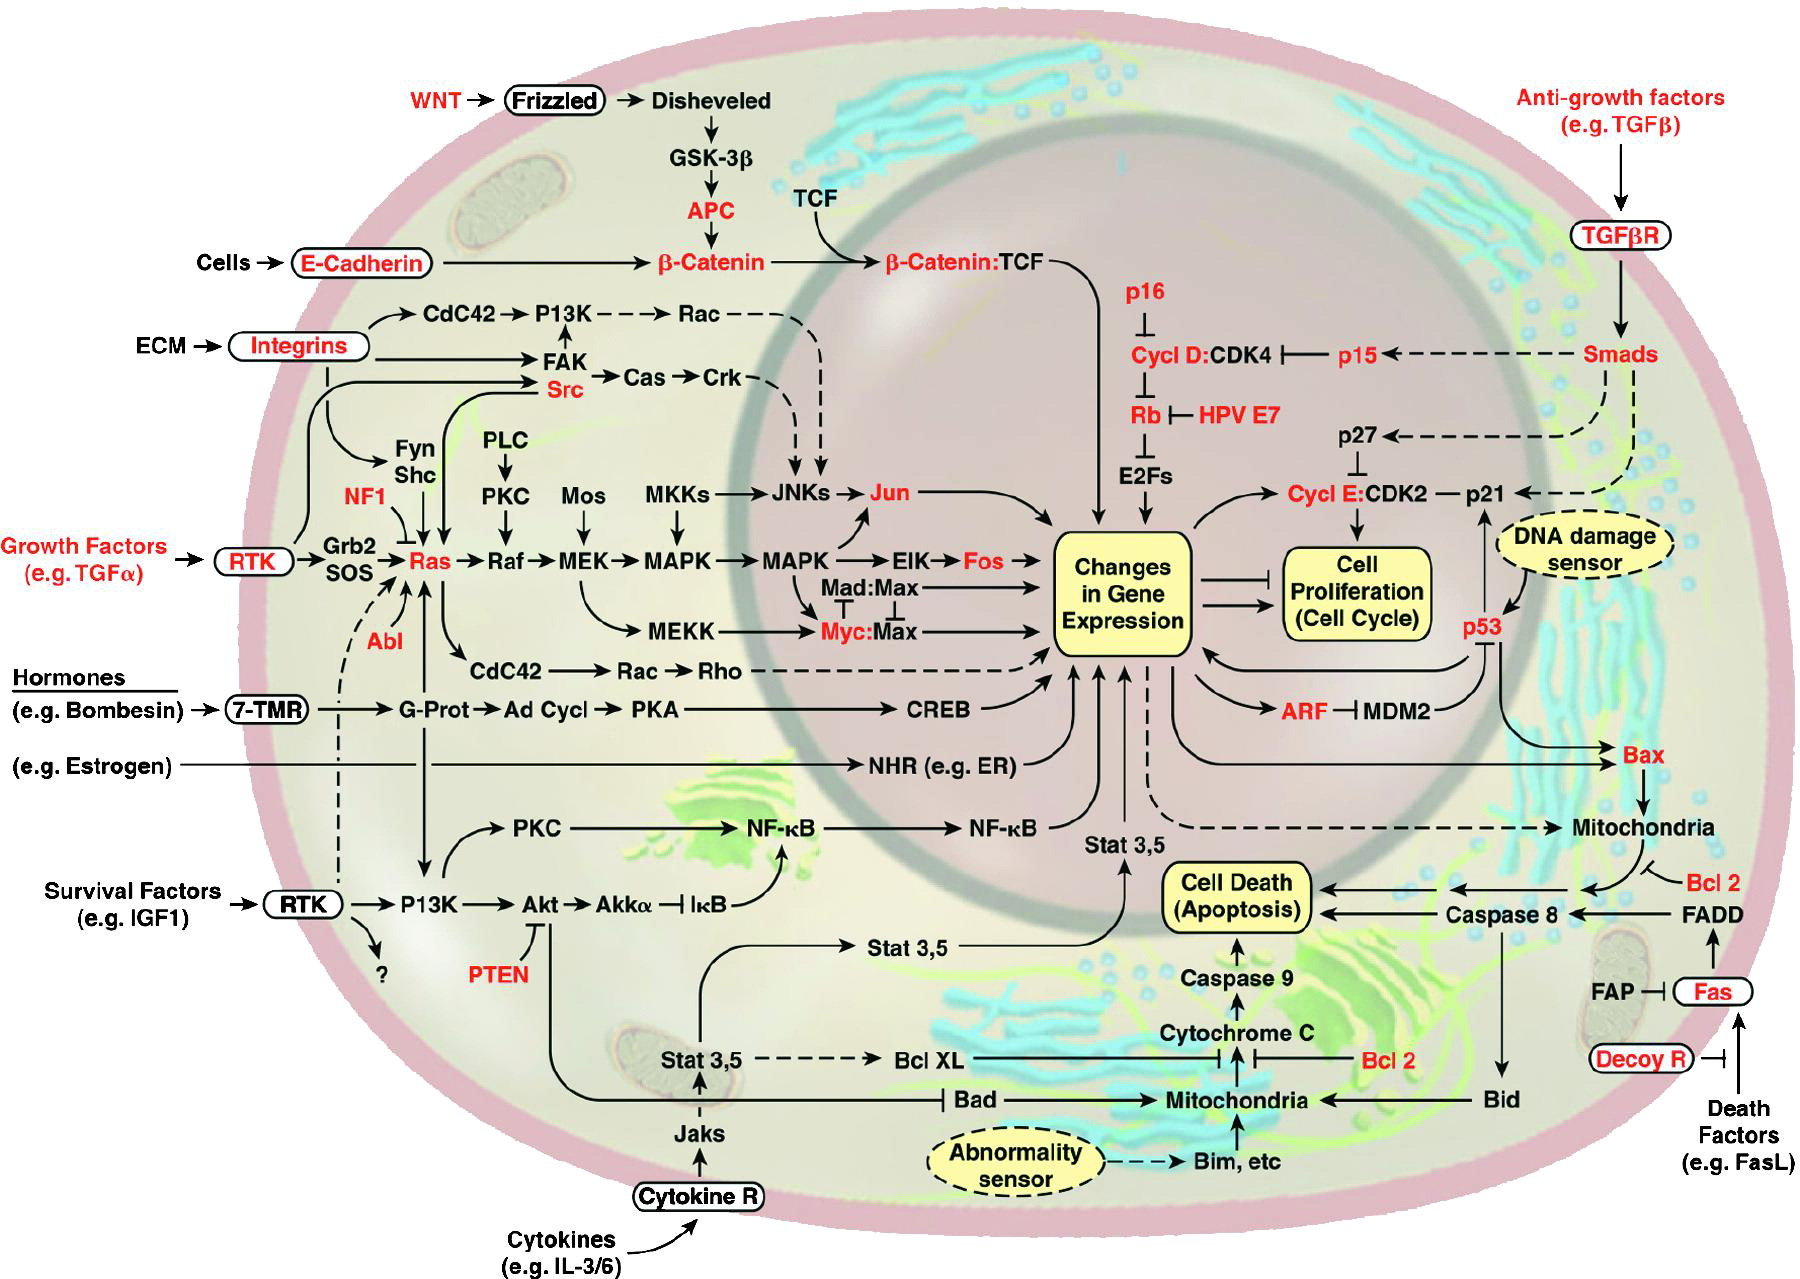
\includegraphics[scale=0.12]{images/cellule-description.jpeg}
\end{center}
\begin{center}
{\tiny \color{darkgreen}[\citelui]}
\end{center}

%\tcite{Wikipédia}

\begin{itemize}
\item Cellular processes $\Longrightarrow$ networks of biological interactions.
\item Nodes (biological components), edges (interactions).
\end{itemize}

%Cellular processes are driven by networks of biological reactions. Cells rely on the tight coordination of these pathways to achieve proper functioning.
%With the help of signaling pathway, a cell senses changes in its environnement or internal state. This information is then passed on via cascades of biochemical 
%reactions to the appropriate mechanisms which respond by modifying the metabolic and transcriptiona activities. this in turn modifies the behavior of the cell.

%Consequently, the dynamics of biopathways play a crucial role in determinig cellular functions.

%Examples: circadian rhythm, the apoptosis pathway inducing programmed cell death, cell differentiation.

%\textcolor{couleurtheme}{$\Rightarrow$} \fbox{\tval{\large The need of comprehension of biological systems}} \textcolor{couleurtheme}{$\Leftarrow$}


%\textcolor{couleurtheme}{$\Rightarrow$} \fbox{\tval{\large Allow efficient translation from Process Hitting to BRN}} \textcolor{couleurtheme}{$\Leftarrow$}

\end{frame}

\begin{frame}[c]
 \frametitle{Motivation}
  %\pause
 %figure illustrative
 \begin{tikzpicture}[auto]

\path[use as bounding box] (-0.7,-2) rectangle (3,3);

%le noeud pour les connaissances de la littérature, générales
\node[align=center] (gk) at (2,3) {\begin{tabular}{|c|}
\hline
 General knowledge  \\
 \hline
 Literature  \\
  \hline
 Hypotheses   \\
  \hline
\end{tabular}};

%\pause

%les noeud pour le réseau biologique
\node[qgre] (a) at (1,1.5) {a};
\node[mod] (i) at (2.3,1) {i};
\node[qgre] (b) at (1,0.5) {b};
\node[qgre] (c) at (3,1) {c};


\path
 (a) edge[act] node[center]{$p_1$\footnotesize ?} (i)
 (b) edge[inh] node[below]{\color{red} $p_2$\footnotesize ?} (i)
 (i) edge[st]  (c);

 %\pause

\node (deco) at (2,-0.1) {Times series data};
\node[align=center] (tsd) at (2,-1) {\begin{tabular}{|c|c|c|c|}
\hline
 Genes  & 1h & ... & 24h  \\
 \hline
 Gene $1$  &   & ...  &    \\
  \hline
  Gene $2$  &   & ...  &    \\
  \hline
\end{tabular}};


\onslide<2->{

\node (d1) at (5,1) {};
\node (d2) at (7.5,1) {};

\node (d3) at (4.5,-1.5) {};
\node (d4) at (4.5,3.5) {};


\draw[->,line width=6pt, color=lightgray] (d1) -- (d2) node[above=10pt,midway]{\textcolor{black}{\textbf{Algebraic Modelling}}};
}

\onslide<2->{
%le modèle en process hitting
\node[scale=0.4] (phmodel) at (10,1) {\begin{tikzpicture} \exphHM
                           \end{tikzpicture}};
}

\end{tikzpicture}

\onslide<2->{
Formal inference of the parameters of Biological Networks:

  \begin{itemize}
   \item Avoid critical behaviors.
  \end{itemize}

}

\end{frame}
                   





\section{Parametric Stochastic Automata Networks}

% Définition du Process Hitting + sortes coopératives

\begin{frame}
  \frametitle{Parametric Stochastic Automata Networks}
  %\framesubtitle{\tcite{Paulev\'e et al. 2012}}


\begin{columns}
\begin{column}{0.6\textwidth}
% 1 : Sortes
\only<1>{
\tikzstyle{process}=[circle,minimum size=15pt,font=\footnotesize,inner sep=1pt]
\tikzstyle{tick label}=[color=white, font=\footnotesize]
\tikzstyle{tick}=[transparent]
\tikzstyle{hit}=[transparent]
\tikzstyle{selfhit}=[transparent, min distance=30pt,curve to]
\tikzstyle{bounce}=[transparent]
\tikzstyle{hlhit}=[transparent]
\tikzstyle{local transitions}=[transparent]
\begin{center}\scalebox{\scaleex}{
\begin{tikzpicture}
\exandef
\end{tikzpicture}
}\end{center}
}

% 2 : Processus
\only<2>{
\tikzstyle{process}=[circle,draw,minimum size=15pt,font=\footnotesize,inner sep=1pt]
\tikzstyle{tick label}=[font=\footnotesize]
\tikzstyle{tick}=[densely dotted]
\tikzstyle{hit}=[transparent]
\tikzstyle{selfhit}=[transparent, min distance=30pt,curve to]
\tikzstyle{bounce}=[transparent]
\tikzstyle{hlhit}=[transparent]
\tikzstyle{local transitions}=[transparent]
\begin{center}\scalebox{\scaleex}{
\begin{tikzpicture}
\exandef
\end{tikzpicture}
}\end{center}
}

% 3 : États
\only<3>{
\tikzstyle{hit}=[transparent]
\tikzstyle{selfhit}=[transparent, min distance=30pt,curve to]
\tikzstyle{bounce}=[transparent]
\tikzstyle{hlhit}=[transparent]
\tikzstyle{local transitions}=[transparent]
\begin{center}\scalebox{\scaleex}{
\begin{tikzpicture}
\exandef

\TState{3}{a_0,b_0,c_0}
\end{tikzpicture}
}\end{center}
}

% 4 : Actions
\only<4->{
\tikzstyle{tick}=[densely dotted]
\tikzstyle{hit}=[->,>=angle 45]
\tikzstyle{selfhit}=[min distance=30pt,curve to]
\tikzstyle{bounce}=[densely dotted,>=stealth',->]
\tikzstyle{hlhit}=[very thick]
\begin{center}\scalebox{\scaleex}{
\begin{tikzpicture}
\exandef
\TState{4}{a_0,b_0,c_0}
\TState{5}{a_1,b_0,c_0}
\TState{6}{a_0,b_0,c_0}
\TState{7}{a_2,b_0,c_0}
\TState{8}{a_2,b_1,c_0}
\end{tikzpicture}
}\end{center}
}
\end{column}

\begin{column}{0.4\textwidth}
\begin{figure}[p]
\centering

\scalebox{0.4}{
\only<4>{
\tikzstyle{arc0}=[transparent]
\tikzstyle{nd0}=[]
\tikzstyle{arc1}=[transparent]
\tikzstyle{nd1}=[transparent]
\tikzstyle{arc2}=[transparent]
\tikzstyle{nd2}=[transparent]
\tikzstyle{arc3}=[transparent]
\tikzstyle{nd3}=[transparent]
\tikzstyle{arc4}=[transparent]
\tikzstyle{nd4}=[transparent]
\tikzstyle{arc5}=[transparent]
\tikzstyle{nd5}=[transparent]
\input{figures/sg-example3.pgf}
}
\only<5>{
\tikzstyle{arc0}=[->]
\tikzstyle{nd0}=[]
\tikzstyle{arc1}=[->]
\tikzstyle{nd1}=[]
\tikzstyle{arc2}=[transparent]
\tikzstyle{nd2}=[transparent]
\tikzstyle{arc3}=[transparent]
\tikzstyle{nd3}=[transparent]
\tikzstyle{arc4}=[transparent]
\tikzstyle{nd4}=[transparent]
\tikzstyle{arc5}=[transparent]
\tikzstyle{nd5}=[transparent]
\input{figures/sg-example3.pgf}
}
\only<6>{
\tikzstyle{arc0}=[->]
\tikzstyle{nd0}=[]
\tikzstyle{arc1}=[->]
\tikzstyle{nd1}=[]
\tikzstyle{arc2}=[->]
\tikzstyle{nd2}=[]
\tikzstyle{arc3}=[transparent]
\tikzstyle{nd3}=[transparent]
\tikzstyle{arc4}=[transparent]
\tikzstyle{nd4}=[transparent]
\tikzstyle{arc5}=[transparent]
\tikzstyle{nd5}=[transparent]
\input{figures/sg-example3.pgf}
}
\only<7>{
\tikzstyle{arc0}=[->]
\tikzstyle{nd0}=[]
\tikzstyle{arc1}=[->]
\tikzstyle{nd1}=[]
\tikzstyle{arc2}=[->]
\tikzstyle{nd2}=[]
\tikzstyle{arc3}=[->]
\tikzstyle{nd3}=[]
\tikzstyle{arc4}=[transparent]
\tikzstyle{nd4}=[transparent]
\tikzstyle{arc5}=[transparent]
\tikzstyle{nd5}=[transparent]
\input{figures/sg-example3.pgf}
}
\only<8>{
\tikzstyle{arc0}=[->]
\tikzstyle{nd0}=[]
\tikzstyle{arc1}=[->]
\tikzstyle{nd1}=[]
\tikzstyle{arc2}=[->]
\tikzstyle{nd2}=[]
\tikzstyle{arc3}=[->]
\tikzstyle{nd3}=[]
\tikzstyle{arc4}=[->]
\tikzstyle{nd4}=[]
\tikzstyle{arc5}=[transparent]
\tikzstyle{nd5}=[transparent]
\input{figures/sg-example3.pgf}
}
\only<9>{
\tikzstyle{arc0}=[->]
\tikzstyle{nd0}=[]
\tikzstyle{arc1}=[->]
\tikzstyle{nd1}=[]
\tikzstyle{arc2}=[->]
\tikzstyle{nd2}=[]
\tikzstyle{arc3}=[->]
\tikzstyle{nd3}=[]
\tikzstyle{arc4}=[->]
\tikzstyle{nd4}=[]
\tikzstyle{arc5}=[->]
\tikzstyle{nd5}=[]
\input{figures/sg-example3.pgf}
}
}

\end{figure}

\end{column}
\end{columns}
%\medskip

\begin{liste}
  \item \tval{Automata}: components \qex{$a$, $b$, $c$}
\pause[2]
  \item \tval{local states}: levels of expression \qex{$c_0$, $c_1$, $c_2$}
\pause[3]
  \item \tval{States}: sets of active local states%
  \only<3-4>{\qex{$\PHetat{a_0, b_0, c_0}$}}%
  \only<5>{\qex{$\PHetat{a_1, b_0, c_0}$}}%
  \only<6>{\qex{$\PHetat{a_0, b_0, c_0}$}}%
  \only<7>{\qex{$\PHetat{a_2, b_0, c_0}$}}%
  \only<8>{\qex{$\PHetat{a_2, b_1, c_0}$}}
\pause[4]
  \item \tval{Transitions}: dynamics \qex{\only<5>{\underline}{$t_1 = \trans{a_0}{a_1}{b_0}$}, \only<6>{\underline}{$t_2 = \trans{a_1}{a_0}{}$}, \only<7>{\underline}{$t_3 = \trans{a_0}{a_2}{b_0,c_0}$}, \only<8>{\underline}{$t_4 = \trans{b_0}{b_1}{}$}}
\end{liste}
%une seule transition à la fois
%on peut avoir un choix il faut bien expliquer ça.
\end{frame}

\begin{comment}
\begin{frame}
  \frametitle{Parametric Stochastic Automata Networks}
  %\framesubtitle{\tcite{Paulev\'e et al. 2012}}
\begin{columns}
\begin{column}{0.6\textwidth}

% Automate sans les rates
\only<1->{
\tikzstyle{tick}=[densely dotted]
\tikzstyle{hit}=[->,>=angle 45]
\tikzstyle{selfhit}=[min distance=30pt,curve to]
\tikzstyle{bounce}=[densely dotted,>=stealth',->]
\tikzstyle{hlhit}=[very thick]
\begin{center}\scalebox{\scaleex}{
\begin{tikzpicture}
\exandef
\end{tikzpicture}
}\end{center}
}
\end{column}

\begin{column}{0.4\textwidth}
\begin{figure}[p]
\centering

\scalebox{0.4}{

\only<1->{
\tikzstyle{arc0}=[->]
\tikzstyle{nd0}=[]
\tikzstyle{arc1}=[->]
\tikzstyle{nd1}=[]
\tikzstyle{arc2}=[->]
\tikzstyle{nd2}=[]
\tikzstyle{arc3}=[->]
\tikzstyle{nd3}=[]
\tikzstyle{arc4}=[->]
\tikzstyle{nd4}=[]
\tikzstyle{arc5}=[->]
\tikzstyle{nd5}=[]
\input{figures/sg-example3.pgf}
}
}

\end{figure}

\end{column}
\end{columns}

\begin{liste}
  \item \tval{Automata}: components \qex{$a$, $b$, $c$}
  \item \tval{local states}: levels of expression \qex{$c_0$, $c_1$, $c_2$}
  \item \tval{States}: sets of active local states%
  \only<1->{\qex{$\PHetat{a_2, b_1, c_0}$}}
  \item \tval{Transitions}: dynamics \qex{\only<1->{$t_1 = \trans{a_0}{a_1}{b_0}$}, \only<1->{$t_2 = \trans{a_1}{a_0}{}$}, \only<1->{$t_3 = \trans{a_0}{a_2}{b_0,c_0}$}, \only<1->{$t_4 = \trans{b_0}{b_1}{}$}}
\end{liste}
\end{frame}
\end{comment}

\begin{frame}
  \frametitle{Parametric Stochastic Automata Networks}
  %\framesubtitle{\tcite{Paulev\'e et al. 2012}}
\begin{columns}
\begin{column}{0.6\textwidth}

% Automate avec les rates
\only<1->{
\tikzstyle{tick}=[densely dotted]
\tikzstyle{hit}=[->,>=angle 45]
\tikzstyle{selfhit}=[min distance=30pt,curve to]
\tikzstyle{bounce}=[densely dotted,>=stealth',->]
\tikzstyle{hlhit}=[very thick]
\begin{center}\scalebox{\scaleex}{
\begin{tikzpicture}
\exsandef
\end{tikzpicture}
}\end{center}
}
\end{column}

\begin{column}{0.4\textwidth}
\begin{figure}[p]
\centering

\scalebox{0.4}{

\only<1->{
\tikzstyle{arc0}=[->]
\tikzstyle{nd0}=[]
\tikzstyle{arc1}=[->]
\tikzstyle{nd1}=[]
\tikzstyle{arc2}=[->]
\tikzstyle{nd2}=[]
\tikzstyle{arc3}=[->]
\tikzstyle{nd3}=[]
\tikzstyle{arc4}=[->]
\tikzstyle{nd4}=[]
\tikzstyle{arc5}=[->]
\tikzstyle{nd5}=[]
\input{figures/sg-example3-rate.pgf}
}
}

\end{figure}

\end{column}
\end{columns}

\begin{liste}
  \item \tval{Automata}: components \qex{$a$, $b$, $c$}
  \item \tval{local states}: levels of expression \qex{$c_0$, $c_1$, $c_2$}
  \item \tval{States}: sets of active local states%
  \only<1->{\qex{$\PHetat{a_2, b_1, c_0}$}}
  \item \tval{Transitions}: dynamics \qex{\only<1->{$t_1 = \trans{a_0}{a_1}{b_0,\mathbf{\color{Maroon} 2}}$}, \only<1->{$t_2 = \trans{a_1}{a_0}{\mathbf{\color{Maroon} 1}}$}, \only<1->{$t_3 = \trans{a_0}{a_2}{b_0,c_0,\mathbf{\color{Maroon} 2}}$}, \only<1->{$t_4 = \trans{b_0}{b_1}{\mathbf{\color{Maroon} 3}}$}}
\end{liste}
\end{frame}






\section{Parameters estimation from time-series data}

\begin{frame}[c]
\frametitle{Approach}
\begin{tikzpicture}[grn]

 % placement des noeuds
 
  \node[block,align=center] (rstc) at (-2,5) {\begin{tabular}{c}
                                            \textbf{Biological network} \\ \hline
                                            RSTC network
                                           \end{tabular}};
  
  \node[block] (data) at (4,5) {\begin{tabular}{c}
                                            \textbf{Experimental Data} \\ \hline
                                            Time series data(TSD)
                                           \end{tabular}};
  
 \node[instruct,align=center] (phmodel) at (-2,2.5) {\begin{tabular}{c}
                                            \textbf{Hybrid Model} \\ \hline
                                            AN Model
                                           \end{tabular}};
                                           
  \node[instruct] (estimation) at (2.5,2.5) {\begin{tabular}{c}
                                            \textbf{Estimation of parameters}\\ \hline
                                            $r$ and $sa$ 
                                           \end{tabular}};
                                           
   
 % \node[instruct] (discretization) at (6.5,2.5) {\begin{tabular}{c}
  %                                          \textbf{Discretization} \\ \hline
   %                                         TSD
    %                                       \end{tabular}};
                                           
  \node[instruct] (simulation) at (-2,0) {\textbf{Simulation}};
    
  
  \node[test] (test) at (3,0) {Model validation};
  
 %placement des arrêtes
  \draw[suite] (rstc) --node[inner,left]{1} (phmodel);
  \draw[suite] (phmodel) --node[inner,left]{4} (simulation);
  \draw[suite] (simulation) --node[inner,above]{5} (test.west);
  
  \draw[suite] (data) --node[inner,left]{2} (estimation);
  \draw[suite] (estimation) --node[inner,above]{3} (phmodel);
  %\draw[suite] (data) --node[inner,left,node distance=5mm]{2'} (discretization);
  %\draw[suite] (discretization) --node[inner,left,node distance=1cm]{5} (test.east);
\end{tikzpicture}

\end{frame}


\begin{frame}[c]
 \frametitle{RSTC Network}
 \framesubtitle{multi-layer receptor-signaling-transcription-cell state}
%\begin{beamer}

\begin{center}
  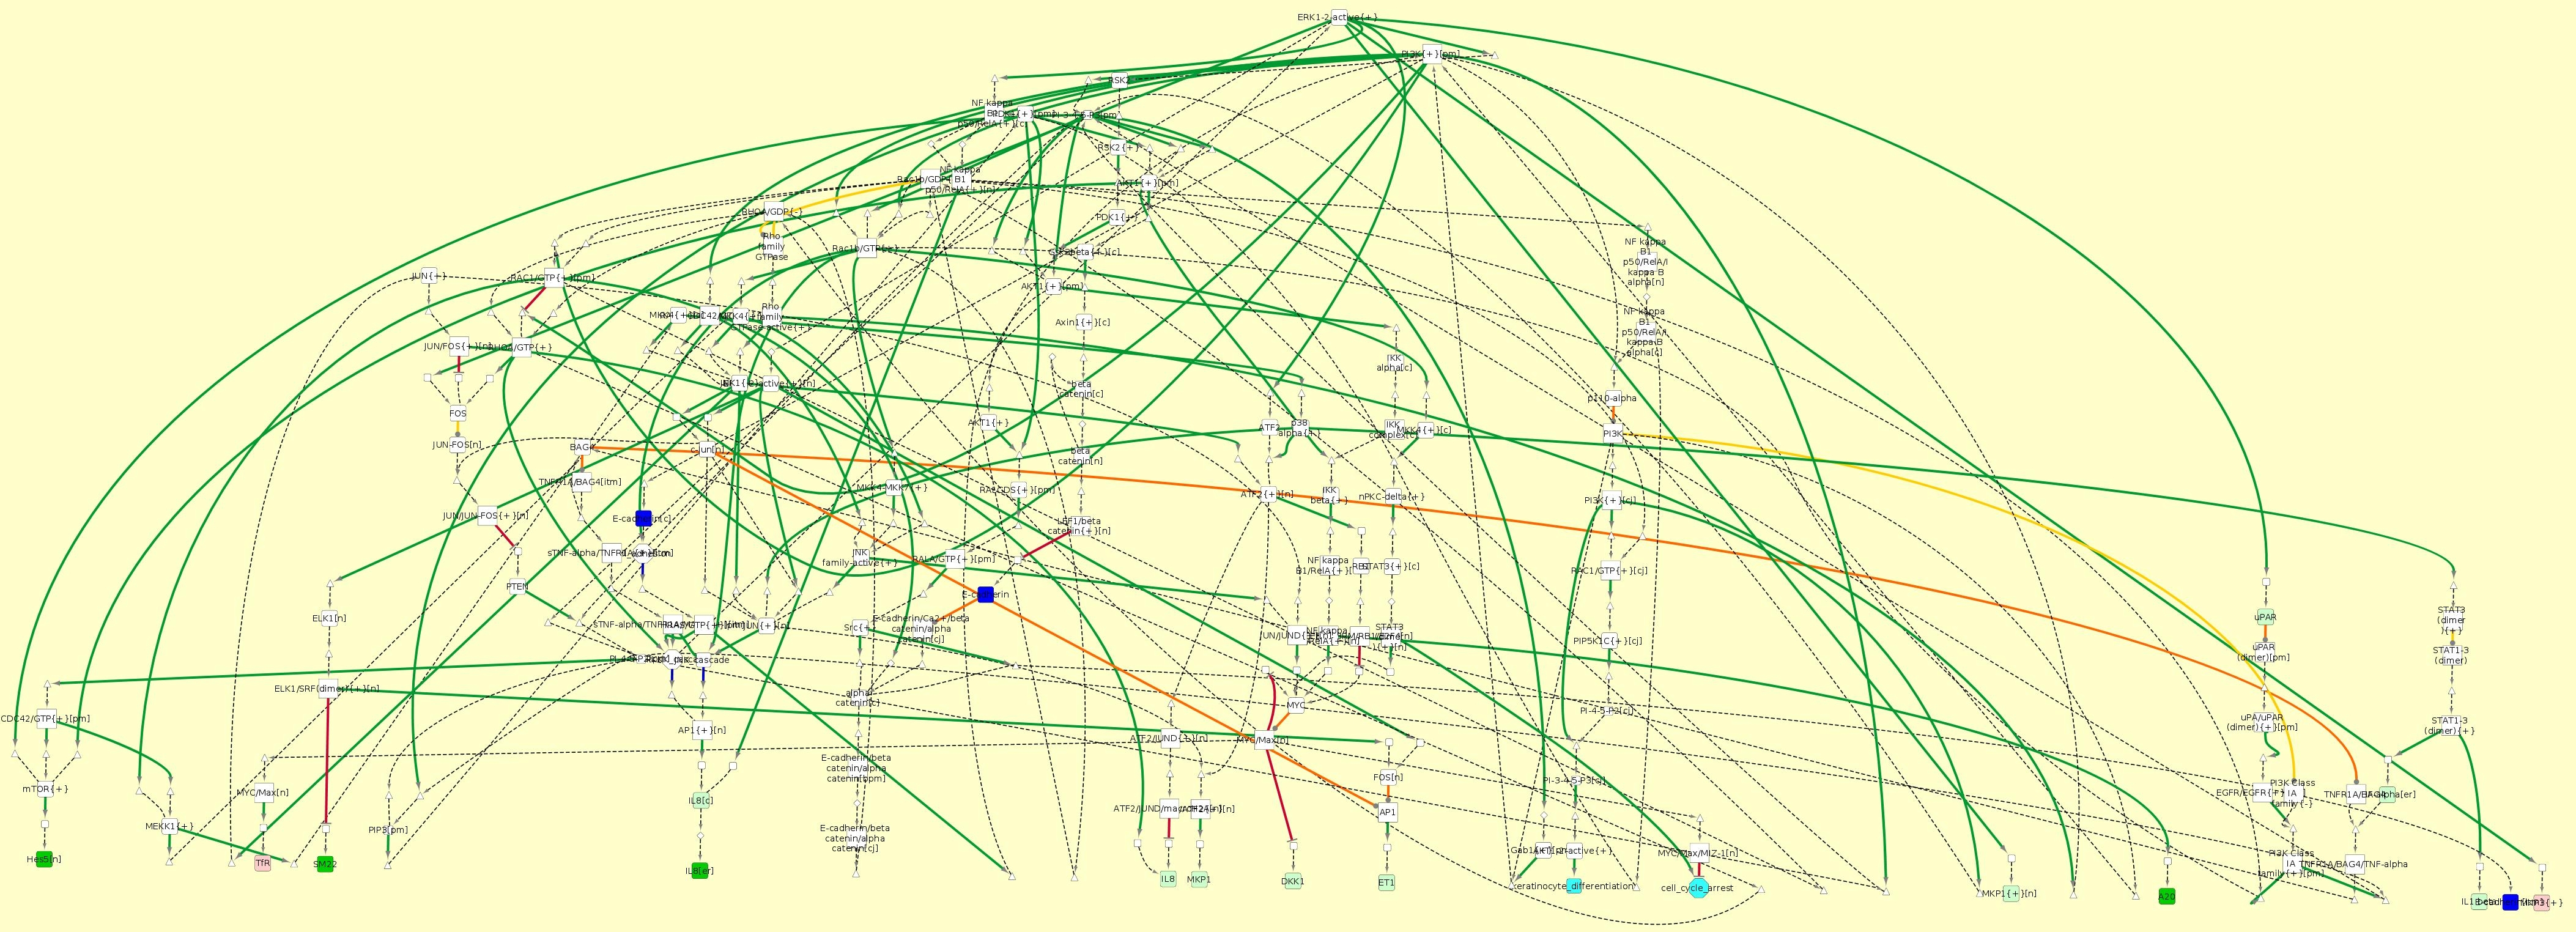
\includegraphics[scale=0.07]{figs/net.jpg}
\end{center}
 
%\end{beamer}

%\pause

\begin{itemize}
 \item Pathway Interaction Database
 \item \tval{$293$  nodes}: signaling proteins, transcription factors, mRNA expressions
 \item \tval{$375$  interactions}: activations, inhibitions, complexes dissociation
\end{itemize}

 
\end{frame}

\begin{frame}[c]
 \frametitle{RSTC Network}
 \framesubtitle{multi-layer receptor-signaling-transcription-cell state}

%%%image zoomée
\begin{tikzpicture}[node distance = 1em,dashed,red,thick]
	\zoomZero{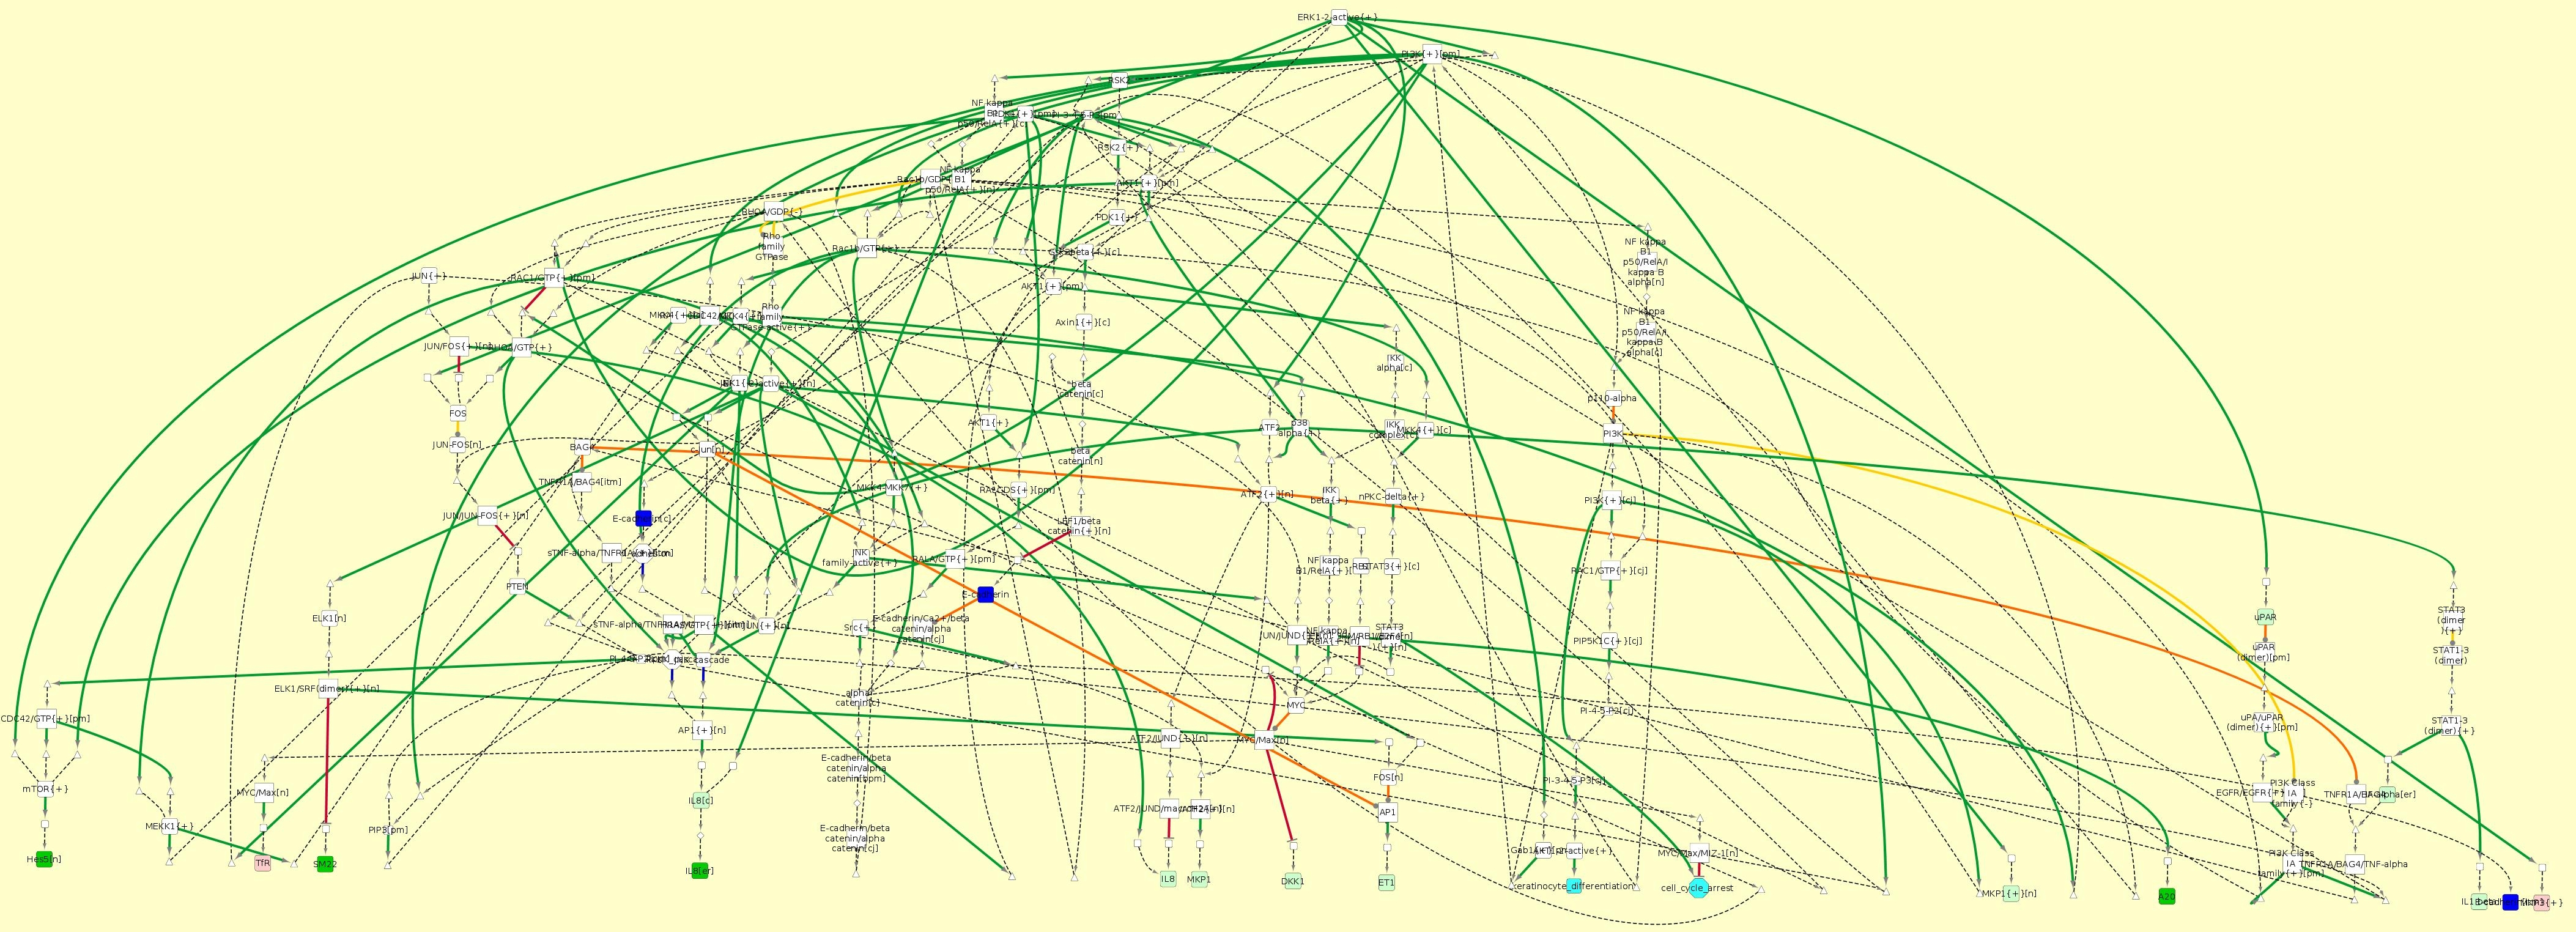
\includegraphics[width=0.35\textwidth]{figs/net.jpg}}
	\zoomIn[right]{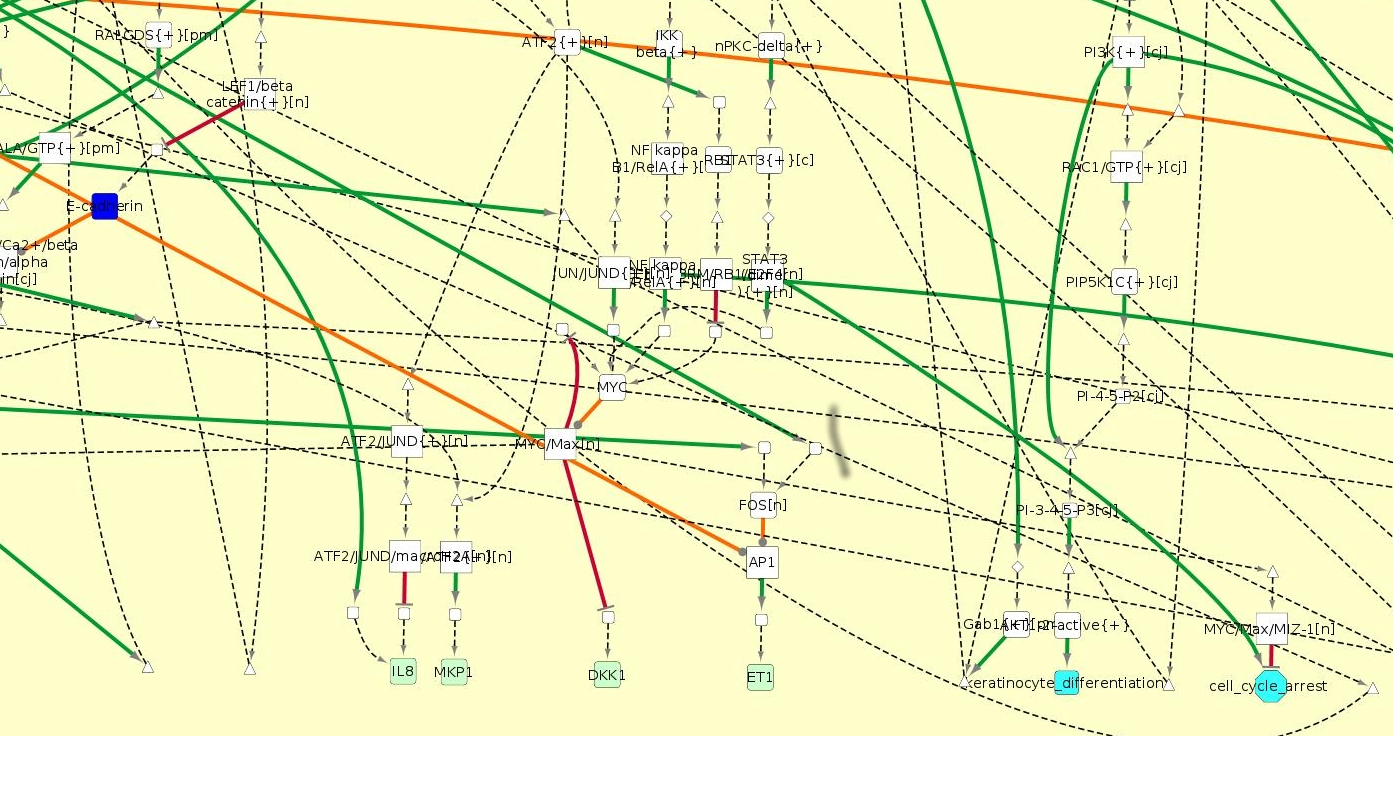
\includegraphics[scale=0.15]{figs/netzoom.png}}{0.35,0.005}{0.320,0.420}
	%\zoomIn{\includegraphics[width=0.45\textwidth]{Geant3}}{0.45,0.475}{0.120,0.120}
	%\zoomIn[left]{\includegraphics[width=0.45\textwidth]{Geant2}}{0.45,0.475}{0.120,0.120}
	%\zoomIn{\includegraphics[width=0.45\textwidth]{Geant1}}{0.45,0.475}{0.120,0.120}
	%\zoomIn[right]{\includegraphics[width=0.45\textwidth]{Geant0}}{0.45,0.475}{0.120,0.120}
\end{tikzpicture}


\end{frame}

\begin{frame}[c]
 \frametitle{RSTC Network}
 \framesubtitle{multi-layer receptor-signaling-transcription-cell state}

%%%image zoomée
\begin{tikzpicture}[node distance = 1em,dashed,red,thick]
	\zoomZero{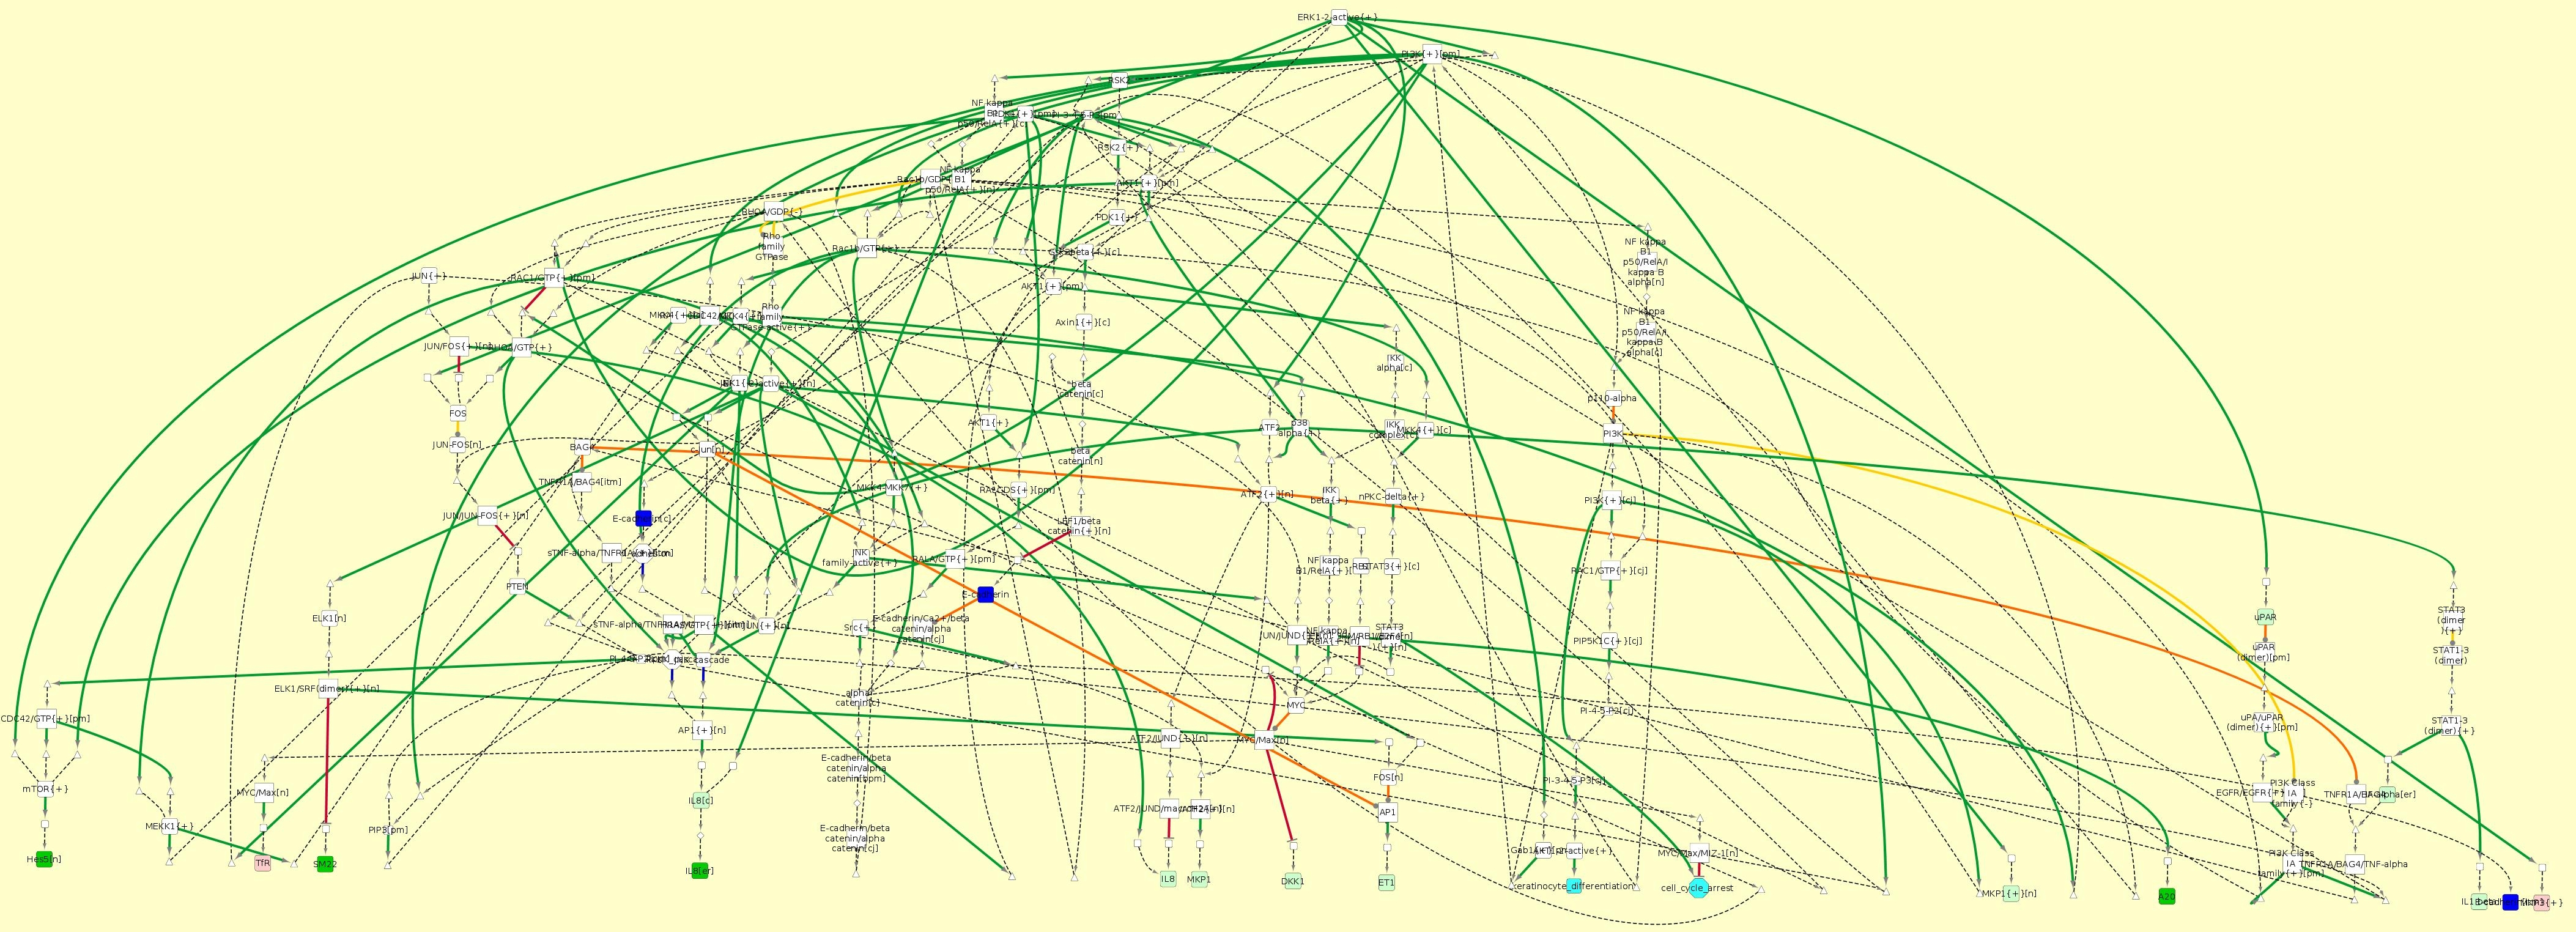
\includegraphics[width=0.45\textwidth]{figs/net.jpg}}
	\zoomIn[left]{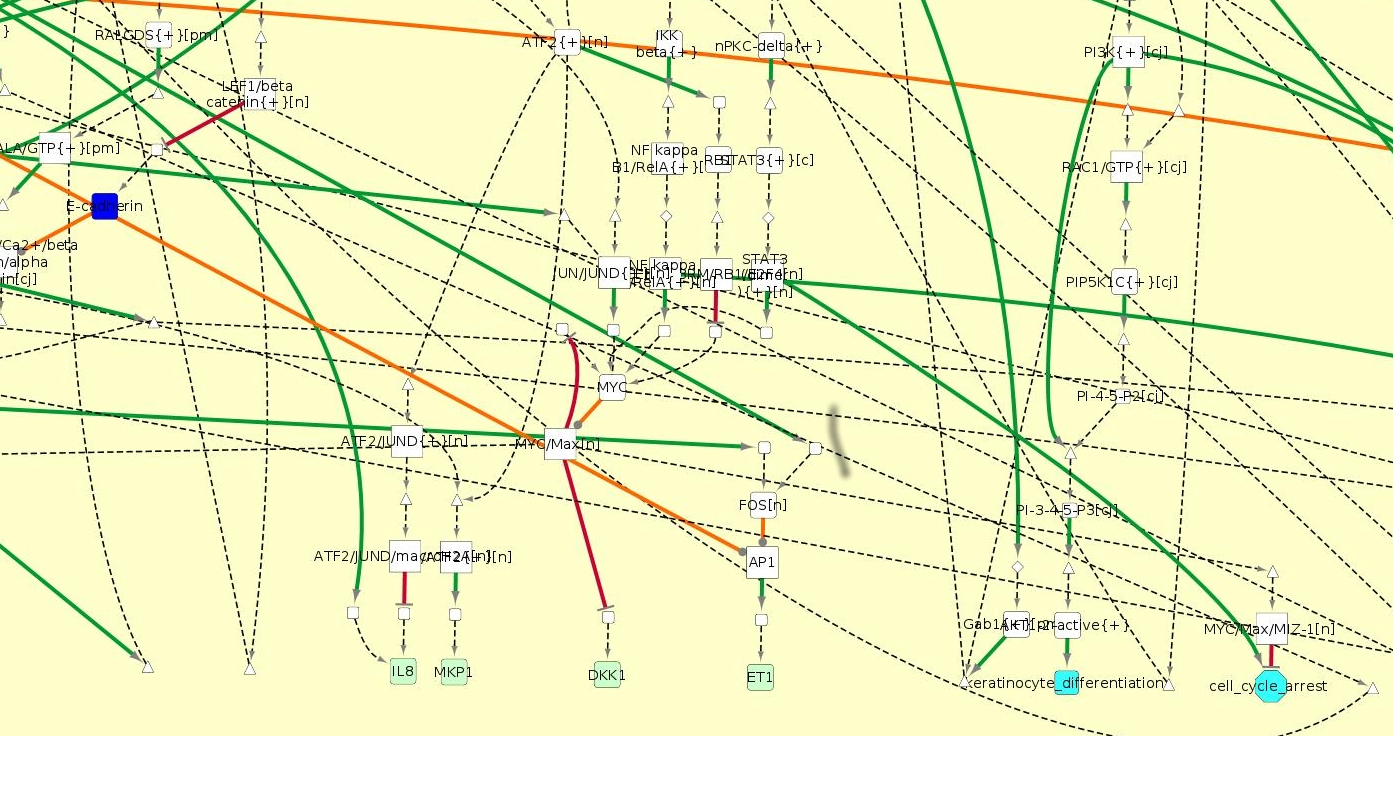
\includegraphics[scale=0.25]{figs/netzoom.png}}{0.35,0.005}{0.320,0.420}
	%\zoomIn{\includegraphics[width=0.45\textwidth]{Geant3}}{0.45,0.475}{0.120,0.120}
	%\zoomIn[left]{\includegraphics[width=0.45\textwidth]{Geant2}}{0.45,0.475}{0.120,0.120}
	%\zoomIn{\includegraphics[width=0.45\textwidth]{Geant1}}{0.45,0.475}{0.120,0.120}
	%\zoomIn[right]{\includegraphics[width=0.45\textwidth]{Geant0}}{0.45,0.475}{0.120,0.120}
\end{tikzpicture}


\end{frame}


\begin{frame}[c]
  \frametitle{Time series data}
  
\begin{center}
  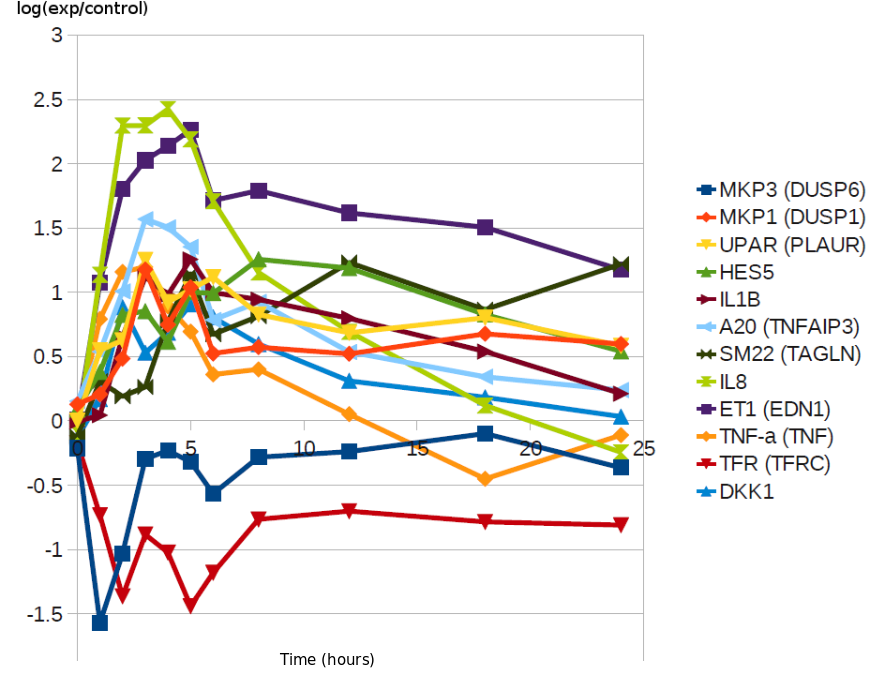
\includegraphics[width=70mm]{figs/12genes.png}
\end{center}

%\pause

\begin{columns}
\begin{column}{0.7\textwidth}
\begin{itemize}
  \item Experiment: \tval{calcium stimuli}
  \item Measured at 10 time-points(0-24hrs)
  \item \tval{$200$ transcripts} selected  (\tval{dynamic patterns}) %their fold expression with respect to the non-stimulated cell was significant in at least one time point
  \item We included in our model a subset of $12$ of them
\end{itemize}
\end{column}

\begin{column}{0.3\textwidth}
% \textbf{ \small Prof. Dr. Peter Angel
%Signal Transduction and Growth Control (A100)
%German Cancer research center
%Heidelberg, Germany}

\end{column}
\end{columns}
%\textcolor{couleurtheme}{$\Rightarrow$} \fbox{\tval{\large Allow efficient translation from Process Hitting to BRN}} \textcolor{couleurtheme}{$\Leftarrow$}

\end{frame}



\begin{frame}[c]
 \frametitle{Data estimation from TSD}
% \framesubtitle{Parameters inference/Principe}
 
\begin{columns}

\begin{column}{0.7\textwidth}
\scalebox{0.9}{
\begin{tikzpicture}[scale = 0.8]
    % Tracé de la parabole
    %\draw[red, domain = -2.2:2.2, smooth] plot (\x, {(\x)^2});
    % Alternative par Gnuplot
    %\draw[red, domain = -2.2:2.2, smooth] plot function{x**2};
    % Lignes tiretées
      \draw[thick, ->] (-.2,0)--(11,0) node[below]{$t$};
     \foreach \t in {0,1,2,3,4,...,10}
      \draw[very thick] (\t,2pt)--(\t,-2pt) node[below,blue]{\small\t};

     \draw[thick, ->] (0,-.2)--(0,4) node[left]{$b$};
     \foreach \y in {1,2,3}
      \draw[very thick] (2pt,\y)--(-2pt,\y) node[left,blue]{\small\y};
      
    \draw[thick] plot[mark=ball,mark size=1pt] file {illustration.txt};
    
    \onslide<2->{
    \draw[thick,|<->|] (2.8,3.5) -- (3.2,3.5) node[above,blue]{$Max$};
    \draw[thick,|<->|] (2.8,-.2) -- (3.2,-.2) node[below,blue]{$Min$};
    }
    \onslide<3->{
    \draw[thick,|<->|] (3,0) -- (3,3.5);
    }
    \onslide<4->{
    \draw[thick,dotted,blue] (0,1.16) -- (10,1.16) node[right]{$th1$}; 
    \draw[thick,dotted,blue] (0,2.33) -- (10,2.33) node[right]{$th2$}; 
    }
    \onslide<5->{
    \draw[thick,dotted,purple] (0.7,1.16) -- (0.7,-.5) node[below]{$t_{1}$};
    }
    \onslide<6->{
    \draw[thick,dotted,purple] (1.5,2.33) -- (1.5,-.3) node[below]{$t_{2}$};
    }
    \onslide<7->{
    \draw[thick,dotted,purple] (4.2,2.33) -- (4.2,-.3) node[below]{$t_{3}$};
    }
    \onslide<8->{
    \draw[thick,dotted,purple] (9.4,1.16) -- (9.4,-.3) node[below]{$t_{4}$};
    }
\end{tikzpicture}
}
%If we assume that $t_{0}=0$,\\
\onslide<5->{$\PHfrappe{a_1}{b_0}{b_1}$ with $r_{1}=\frac{1}{t_{1}-t_{0}}$\\}
\onslide<6->{$\PHfrappe{a_1}{b_1}{b_2}$ with $r_{2}=\frac{1}{t_{2}-t_{1}}$\\}
\onslide<7->{$\PHfrappe{a_0}{b_2}{b_1}$ with $r_{3}=\frac{1}{t_{3}-t_{2}}$\\}
\onslide<8->{$\PHfrappe{a_0}{b_1}{b_0}$ with $r_{4}=\frac{1}{t_{4}-t_{3}}$\\}
\onslide<8->{The formula to estimate the rate of the dynamics of a component according to it TSD is 
\tval{ \Large {$r_{i}=\frac{1}{t_{i}-t_{i-1}}$}}}
\end{column}

\begin{column}{0.3\textwidth}
\scalebox{0.9}{
 \begin{tikzpicture}[scale=0.8]
\path[use as bounding box] (-1,-1) rectangle (2,2);


\TSort{(0,1)}{b}{3}{r}


\only<5->{\TSort{(2,1)}{a}{2}{l}}
\only<5>{
\THit{a_1}{}{b_0}{.east}{b_1}
%\THit{a_0}{out=-120,in=180,selfhit}{a_0}{.west}{a_1}
\path[bounce]
%\TBounce{a_0}{bend left}{a_1}{.south}
\TBounce{b_0}{bend right}{b_1}{.south}
;
\TState{5}{a_1,b_0}
\TState{5}{a_1,b_1}
}

%deuxième estimation
\only<6>{
\THit{a_1}{}{b_1}{.east}{b_2}
%\THit{a_0}{out=-120,in=180,selfhit}{a_0}{.west}{a_1}
\path[bounce]
%\TBounce{a_0}{bend left}{a_1}{.south}
\TBounce{b_1}{bend right}{b_2}{.south}
;
\TState{6}{a_1,b_1}
\TState{6}{a_1,b_2}
}

%troisième  estimation
\only<7>{
\THit{a_0}{}{b_2}{.east}{b_1}
%\THit{a_0}{out=-120,in=180,selfhit}{a_0}{.west}{a_1}
\path[bounce]
%\TBounce{a_0}{bend left}{a_1}{.south}
\TBounce{b_2}{bend right}{b_1}{.north}
;
\TState{7}{a_0,b_2}
\TState{7}{a_0,b_1}
}

%troisième  estimation
\only<8>{
\THit{a_0}{}{b_1}{.east}{b_0}
%\THit{a_0}{out=-120,in=180,selfhit}{a_0}{.west}{a_1}
\path[bounce]
%\TBounce{a_0}{bend left}{a_1}{.south}
\TBounce{b_1}{bend right}{b_0}{.north}
;
\TState{8}{a_0,b_1}
\TState{8}{a_0,b_0}
}

\end{tikzpicture}
}

\end{column}
\end{columns}
\end{frame}







\begin{frame}[c]
  \frametitle{Simulations and analysis}
  
 \begin{center}
  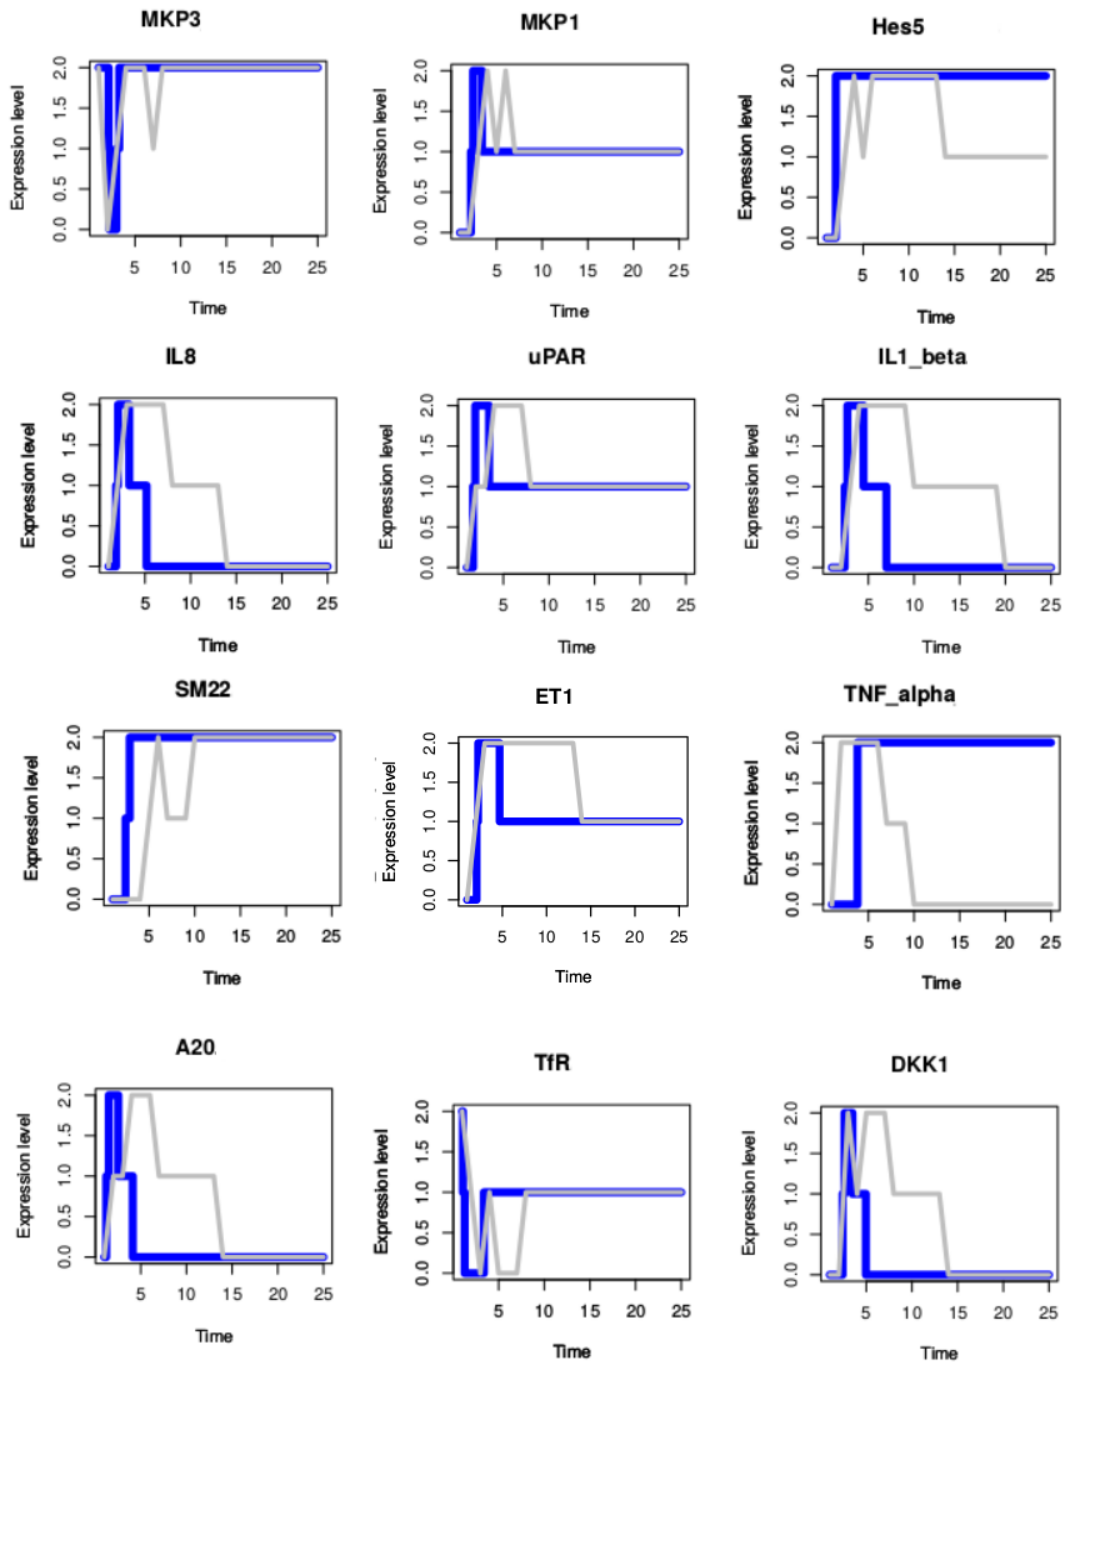
\includegraphics[scale=0.15]{figs/12genes_sim.png}
\end{center}

\textbf{Simulations}

\begin{itemize}
  \item For $r_{a} = r_{i}=10.0$ et $sa = 50 $ for all signalling proteins
  \item With estimated $r$ and $sa$ for MKP3, MKP1, uPAR, Hes5,... according to their expression profiles
  
\end{itemize}

%\textcolor{couleurtheme}{$\Rightarrow$} \fbox{\tval{\large Analyse???}} \textcolor{couleurtheme}{$\Leftarrow$}

\end{frame}




\begin{frame}[c]
  \frametitle{Simulations and analysis}
  
 \begin{center}
  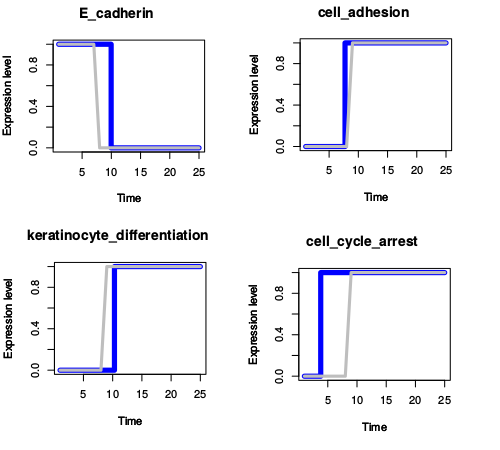
\includegraphics[scale=0.35]{figs/key_nodes1.png}
\end{center}

\textbf{Simulations}

\begin{itemize}
  \item Input node of the system (E\_cadherin)
 \item For biological processes (Cell adhesion, Cell cycle arrest, Keratinocyte differentiation)
  
\end{itemize}

%\textcolor{couleurtheme}{$\Rightarrow$} \fbox{\tval{\large Analyse???}} \textcolor{couleurtheme}{$\Leftarrow$}

\end{frame}


\begin{frame}
   \frametitle{Simulation and Trace analysis}
   %\framesubtitle{work with Guillaume Taupiac}


\begin{columns}
\begin{column}{0.5\textwidth}

\scalebox{0.9}{
\begin{tikzpicture}[scale = 0.8]
       
    \draw[thick, ->] (-.2,-.1)--(7,-.1) node[below]{$t$};
     \foreach \t in {1,2,3,4,5,6}
      \draw[very thick] (\t,-1pt)--(\t,-2pt) node[below,blue]{\small\t};

     \draw[thick, ->] (0,-.2)--(0,3) node[left]{$Level$};
     \foreach \y in {0,1,2}
      \draw[very thick] (2pt,\y)--(-2pt,\y) node[left,blue]{\small\y};
    
    
    \draw[thick,dotted,blue] (0,0) -- (2,0) node[below]{}; 
    \draw[thick,dotted,blue] (2,0) -- (2,1) node[below]{}; 
    \draw[thick,dotted,blue] (2,1) -- (4,1) node[below]{};
    \draw[thick,dotted,blue] (4,1) -- (4,0) node[below]{};
    \draw[thick,dotted,blue] (4,0) -- (6,0) node[below]{};
    \node[instruct,align=center] (mot2) at (4,2) {$\omega=010$};

\end{tikzpicture}
}


%deuxième exemple 
\scalebox{0.9}{
\begin{tikzpicture}[scale = 0.8]
       
    \draw[thick, ->] (-.2,-.1)--(7,-.1) node[below]{$t$};
     \foreach \t in {1,2,3,4,5,6}
      \draw[very thick] (\t,-1pt)--(\t,-2pt) node[below,blue]{\small \t};

     \draw[thick, ->] (0,-.2)--(0,3) node[left]{$Level$};
     \foreach \y in {0,1,2}
      \draw[very thick] (2pt,\y)--(-2pt,\y) node[left,blue]{\small \y};
    
    
    \draw[thick,dotted,blue] (0,0) -- (1,0) node[below]{}; 
    \draw[thick,dotted,blue] (1,0) -- (1,1) node[below]{}; 
    \draw[thick,dotted,blue] (1,1) -- (2,1) node[below]{};
    \draw[thick,dotted,blue] (2,1) -- (2,2) node[below]{};
    \draw[thick,dotted,blue] (2,2) -- (3,2) node[below]{};
    \draw[thick,dotted,blue] (3,2) -- (3,1) node[below]{};
    \draw[thick,dotted,blue] (3,1) -- (5,1) node[below]{};
    \draw[thick,dotted,blue] (5,1) -- (5,0) node[below]{};
    \draw[thick,dotted,blue] (5,0) -- (6,0) node[below]{};
    \node[instruct,align=center] (mot2) at (5,2) {$\omega=01210$};
   

\end{tikzpicture}
}


\end{column}


\begin{column}{0.5\textwidth}

for each component \tval{$C_{i}$, $1 \leq i \leq P$},
\tval{$N$} simulations will generate \tval{$\omega_{i1}, \omega_{i2}, \ldots ,\omega_{iN}$} words.




for $1 \leq j \leq N$

%\newline
%\vspace{1cm}



\scalebox{0.9}{
\begin{tikzpicture}[scale = 0.8]
    
    \node[align=center,blue] (mot) at (2,3) {$\omega_{ij} \Rightarrow $};
    
    \draw[blue] (3,2) rectangle (7,4);

    \node[align=center] (automaton) at (5,3) {$\mathcal{A}_{C_{i}}$};
    
    \node[align=center] (accept) at (8,3) {$\Rightarrow \tval{yes}/\alert{no} $};
    
    \node[align=center] (percent) at (5,1) {\tval{$\% of Acceptance = \frac{\card{YES}}{\card{Simulations}}$}};
   

\end{tikzpicture}
}



\end{column}
\end{columns}
\end{frame}

\begin{frame}
\frametitle{Simulation and Trace analysis}
\begin{tabular}{|c|c||c|c|}
\hline

\textbf{Automate} & \textbf{components} & \textbf{$\%$  validation} & \textbf{$\%$ of acceptance $T_{1}$}
\\ \hline

$\mathcal{A}_{2}(01210)$ & A20 & 91 & 100 
\\ \hline

$\mathcal{A}_{2}(01210)$ & IL1$\_$beta & 81 & 100
\\ \hline

$\mathcal{A}_{2}(01210)$ & IL8 & 93 & 100 
\\ \hline

$\mathcal{A}_{2}(01210)$ & TNF$\_$alpha & 0 & 0
\\ \hline

$\mathcal{A}_{3}(01211)$ & uPar & 76 & 99 
\\ \hline

$\mathcal{A}_{3}(01211)$ & ET1 & 8 & 19 
\\ \hline

$\mathcal{A}_{4}(0121210)$ & DKK1 & 13 & 43

\\ \hline

$\mathcal{A}_{5}(0121211)$ & Hes5 & 0 & 17 
\\ \hline

$\mathcal{A}_{5}(0121211)$ & MKP1 & 9 & 97
\\ \hline

$\mathcal{A}_{6}(0212)$ & SM22 & 11 & 100 
\\ \hline

$\mathcal{A}_{7}(02010)$ & MKP3 & 11 & 98

\\ \hline

$\mathcal{A}_{8}(02121)$ & Tfr & 0 & 94 
\\ \hline

\end{tabular}

\end{frame}




\section{Formal inference of parameters}

\begin{frame}
\frametitle{Formal inference of parameters}


\end{frame}


\section{Discussion}

\begin{frame}
\frametitle{Discussion}

\end{frame}



\begin{frame}[plain,label=title]

% Cadre de titre
\begin{center}
\vspace{1cm}
\setbeamercolor{postit}{fg=black,bg=colortitle}
\begin{beamercolorbox}[sep=0.5em]{postit}
\centering
\Large
\textbf{%
{\normalsize\theconference{}}\\~\\%
\inserttitle
}
\end{beamercolorbox}

% Auteurs et instituts
% Auteurs et instituts


\par
\medskip
\normalsize
Louis Fippo Fitime$^1$
\footnotesize

\texttt{fippofitime@lipn.univ-paris13.fr}

\url{http://www.irccyn.ec-nantes.fr/~fippofit/}



\bigskip
\textbf{Joint work with:} \\  \'Etienne Andr\'e$^1$ and Laure Petrucci$^1$

% Auteurs et instituts

\medskip
\footnotesize
$^1$ LCR / LIPN / CNRS (Paris, France)

\texttt{etienne.andre@lipn.fr}

\texttt{laure.petrucci@lipn.univ-paris13.fr}


\end{center}

Thank you for your attention!!!

\end{frame}



\end{document}


